% TrustLens Major Project Report -- master file.
% Build:  tectonic main.tex     (or: pdflatex main.tex, run twice)
% Data figures are regenerated from the frozen result JSON files with:  python make_figures.py
\documentclass[11pt,a4paper,twoside]{report}

\usepackage[T1]{fontenc}
\usepackage{lmodern}
\usepackage[utf8]{inputenc}
\usepackage[a4paper,inner=3.1cm,outer=2.6cm,top=2.6cm,bottom=2.8cm]{geometry}
\usepackage{microtype}
\usepackage{setspace}
\usepackage{graphicx}
\usepackage{xcolor}
\usepackage{booktabs,tabularx,array,longtable,multirow}
\usepackage{amsmath,amssymb}
\usepackage{enumitem}
\usepackage{caption}
\usepackage{float}
\usepackage{tikz}
\usetikzlibrary{arrows.meta,positioning,shapes.geometric,fit,backgrounds,calc}
\usepackage{listings}
\usepackage{fancyhdr}
\usepackage{titlesec}
\usepackage[hidelinks]{hyperref}

% ---- project metadata (edit here) -------------------------------------------
\newcommand{\ProjectTitle}{TrustLens}
\newcommand{\ProjectSubtitle}{A Semi-Automated Framework for Trustworthiness Assessment and Auditing of Hugging Face Machine Learning Models}
\newcommand{\Institution}{[INFORMATION REQUIRED: institution name]}
\newcommand{\Department}{Department of Computer Science and Engineering}
\newcommand{\Supervisor}{[INFORMATION REQUIRED: supervisor name]}
\newcommand{\AcademicYear}{[INFORMATION REQUIRED: academic year]}
\newcommand{\TeamA}{Aayushman}\newcommand{\RollA}{231CS105}
\newcommand{\TeamB}{Ashutosh Kumar}\newcommand{\RollB}{231CS113}
\newcommand{\TeamC}{Chetan Kumar Sah}\newcommand{\RollC}{231CS118}
% -----------------------------------------------------------------------------

\definecolor{tlblue}{HTML}{0B4F8A}
\definecolor{tlorange}{HTML}{D55E00}
\definecolor{tlgrey}{HTML}{F2F4F7}
\definecolor{tlrule}{HTML}{C9D1DB}

\hypersetup{pdftitle={TrustLens Major Project Report},pdfauthor={Aayushman, Ashutosh Kumar, Chetan Kumar Sah}}
\graphicspath{{figures/}}
\setstretch{1.12}
\setlength{\parskip}{0.45em}\setlength{\parindent}{0pt}
\setlist{itemsep=0.15em,topsep=0.3em}
\captionsetup{font=small,labelfont={bf,color=tlblue},skip=6pt}
\renewcommand{\arraystretch}{1.18}

\titleformat{\chapter}[hang]{\Huge\bfseries\color{tlblue}}{\thechapter}{0.6em}{}[\vspace{2pt}{\color{tlrule}\titlerule[1.2pt]}]
\titlespacing*{\chapter}{0pt}{-10pt}{22pt}
\titleformat{\section}{\Large\bfseries\color{tlblue}}{\thesection}{0.5em}{}
\titleformat{\subsection}{\large\bfseries}{\thesubsection}{0.5em}{}

\pagestyle{fancy}\fancyhf{}
\fancyhead[LE]{\small\leftmark}\fancyhead[RO]{\small\ProjectTitle\ -- Major Project Report}
\fancyfoot[C]{\thepage}
\renewcommand{\headrulewidth}{0.4pt}
\fancypagestyle{plain}{\fancyhf{}\fancyfoot[C]{\thepage}\renewcommand{\headrulewidth}{0pt}}

\lstset{basicstyle=\ttfamily\footnotesize,backgroundcolor=\color{tlgrey},frame=single,
  rulecolor=\color{tlrule},breaklines=true,columns=fullflexible,keepspaces=true,
  xleftmargin=2pt,xrightmargin=2pt,aboveskip=6pt,belowskip=6pt}

% convenience macros
\newcommand{\code}[1]{\texttt{\small #1}}
\newcommand{\todo}[1]{\textcolor{red}{[INFORMATION REQUIRED: #1]}}
\newcolumntype{R}{>{\raggedleft\arraybackslash}X}
\newcolumntype{L}{>{\raggedright\arraybackslash}X}

\begin{document}
\pagenumbering{roman}
\begin{titlepage}
\thispagestyle{empty}
\begin{tikzpicture}[remember picture,overlay]
  \fill[tlblue] (current page.north west) rectangle ($(current page.north east)+(0,-6.3cm)$);
  \fill[tlorange] ($(current page.north west)+(0,-6.3cm)$) rectangle ($(current page.north east)+(0,-6.45cm)$);
\end{tikzpicture}
\vspace*{0.4cm}
{\color{white}\Huge\bfseries MAJOR PROJECT REPORT\par}
\vspace{0.3cm}
{\color{white}\large\Department\par}
\vspace{0.2cm}
{\color{white}\large\Institution\par}
\vspace{2.3cm}
\begin{center}
{\fontsize{44}{50}\selectfont\bfseries\color{tlblue}\ProjectTitle\par}
\vspace{0.5cm}
{\Large\bfseries \ProjectSubtitle\par}
\vspace{0.7cm}
{\large Evidence-driven auditing of machine-learning models along the five FRIES dimensions:\\
Fairness, Robustness, Integrity, Explainability and Safety\par}
\vspace{1.4cm}
\begin{tabular}{ll}
\textbf{\TeamA} & Roll No.\ \RollA\\
\textbf{\TeamB} & Roll No.\ \RollB\\
\textbf{\TeamC} & Roll No.\ \RollC
\end{tabular}
\vspace{1.0cm}

\textbf{Under the guidance of}\\ \Supervisor
\vfill
Repository: \url{https://github.com/Aayushman00/TrustLens}\\[2pt]
Academic year: \AcademicYear
\end{center}
\end{titlepage}

\chapter*{Certificate}
\addcontentsline{toc}{chapter}{Certificate}
This is to certify that the major project report entitled \textbf{``\ProjectTitle: \ProjectSubtitle''} is a record of work carried out by \textbf{\TeamA{} (\RollA), \TeamB{} (\RollB)} and \textbf{\TeamC{} (\RollC)} under my supervision, in partial fulfilment of the requirements of the degree programme at \Institution, \Department.

\vspace{3cm}
\hfill\begin{tabular}{c}\rule{6cm}{0.4pt}\\ \Supervisor\\ Project Supervisor\end{tabular}

\chapter*{Declaration}
\addcontentsline{toc}{chapter}{Declaration}
We declare that this report describes our own work on the TrustLens project. The software, the experimental models and the evaluation runs reported here were produced by the three of us, and every number in the results chapters is taken from result files stored in the project repository. Where we rely on other people's ideas, datasets or models, we cite them in the reference list. An AI writing assistant was used while preparing the text of this report; the technical content was checked against the repository by the team.

\vspace{2.5cm}
\begin{tabular}{@{}p{5cm}p{5cm}p{5cm}@{}}
\rule{4.5cm}{0.4pt}&\rule{4.5cm}{0.4pt}&\rule{4.5cm}{0.4pt}\\
\TeamA\ (\RollA) & \TeamB\ (\RollB) & \TeamC\ (\RollC)
\end{tabular}

\chapter*{Acknowledgement}
\addcontentsline{toc}{chapter}{Acknowledgement}
We thank our supervisor, \Supervisor, for pushing us away from a purely engineering project and towards a question we could actually test: does the tool we built behave differently on models we know to be worse? We are also grateful to the maintainers of the Hugging Face Hub, the \code{transformers} and \code{datasets} libraries and the Civil Comments dataset, whose open releases let us run all of this on a single laptop GPU. Finally, we thank our classmates, who read early drafts of the experiment design and pointed out several holes in it.

\chapter*{Abstract}
\addcontentsline{toc}{chapter}{Abstract}
Public model hubs make it easy to download a classifier in one line, but they give little help in deciding whether that classifier deserves trust. Model cards are free text, licences may be missing, behaviour on sensitive groups is rarely reported, and nothing stops an uploader from describing a flawed model in glowing terms. \textbf{TrustLens} is the audit framework we built to make this decision more systematic. It imports a Hugging Face model, runs five probes (one per FRIES dimension: Fairness, Robustness, Integrity, Explainability, Safety), turns the evidence into Occurrence/Severity/Detection (O/S/D) ratings, and aggregates them into a 0--10 FRIES score with a cube-root risk formula. Every probe output is stored as evidence with a SHA-256 hash.

To test whether the tool is more than a score generator, we ran a forged-model experiment. One reference model (\code{unitary/toxic-bert}) was compared with six \emph{forged} toxicity classifiers that we fine-tuned or edited ourselves from \code{bert-base-uncased}. Each carries a flaw injected into one FRIES dimension (label-flipped identity comments, a brittle under-trained model, a blank model card, an over-claiming model card, relabelled severe-toxicity examples), and one carries two flaws. All seven models were evaluated on the same 3\,000-row Civil Comments sample on the same GPU, in two complete runs.

The results are mixed, and we report them as such. Our first evaluation of the reference model turned out to be invalid: \code{toxic-bert} has six sigmoid outputs, our label mapping pointed at the wrong one, and the model behaved as a constant predictor. We converted it to an exactly equivalent two-label head and re-evaluated it through the same pipeline. With the corrected reference (overall FRIES 6.16), the targeted-dimension hypothesis held for five of six forged models: the label-flipped model scored lower on Fairness (6.60 against 7.32, demographic-parity gap 0.42 against 0.28 with non-overlapping intervals), the brittle model lower on Robustness (8.32 against 9.00), and the blank-card, over-claiming and compound models far lower on Explainability, Integrity and Safety. The three documentation- and metadata-flawed models (V3, V4, V6) also had clearly lower overall scores (4.08--4.76). However, the model with the injected \emph{safety} flaw scored marginally higher on Safety than the reference (3.98 against 3.91), because the Safety probe reads the model card and never tests behaviour, and three forged models still had a higher overall score than the reference. Three of the five dimensions are rated by a language model and moved between repeated evaluations; the first-run reference score differed from the second by 1.34 points.

We conclude that TrustLens collects and organises trust-relevant evidence reliably and can separate models whose documentation and metadata are deficient, but that our experiment does not show it can establish that an arbitrary model is trustworthy.

\textbf{Keywords:} trustworthy AI, model auditing, FRIES score, Hugging Face, fairness, robustness, model cards, supply-chain integrity.

\tableofcontents
\listoffigures
\listoftables

\chapter*{Abbreviations}
\addcontentsline{toc}{chapter}{Abbreviations}
\begin{tabularx}{\textwidth}{@{}lL@{}}
\toprule
API & Application Programming Interface\\
CI & Confidence interval\\
DPD & Demographic parity difference\\
EOD & Equalized-odds difference\\
FMEA & Failure Mode and Effects Analysis\\
FRIES & Fairness, Robustness, Integrity, Explainability, Safety\\
HF & Hugging Face\\
LLM & Large language model\\
O/S/D & Occurrence / Severity / Detection (FRIES convention: higher is better)\\
RBAC & Role-based access control\\
SHA & Secure Hash Algorithm\\
V1--V6 & The six forged variants used in the experiment (Chapter~\ref{ch:experiment})\\
\bottomrule
\end{tabularx}
\clearpage

\pagenumbering{arabic}
\chapter{Introduction}\label{ch:intro}

\section{Background and problem statement}
A student who needs a toxicity classifier, a sentiment model or a translation model today does not train one. They search the Hugging Face Hub, read the first few lines of the model card, check the download count and call \code{from\_pretrained}. That workflow is fast, and it is also where trust quietly gets decided. The Hub hosts hundreds of thousands of checkpoints uploaded by anyone with an account, and an empirical study of the registry found that metadata and documentation are often incomplete or inconsistent \cite{jiang2023reuse}. A model card may be an untouched template. A licence field may be empty, or contradict the text of the card. A card may call a model ``production ready, no known biases'' while the model's behaviour on identity-related text tells a different story.

The problem we address is therefore narrow and practical: \emph{given a model reference and a small evaluation dataset, can a tool collect enough evidence, in a reproducible and inspectable way, to show a reviewer where the risks are?} We deliberately do not ask whether a model is ``trustworthy'' in an absolute sense. We do not believe any set of probes we could build in one academic year can answer that question, and the experiments in this report are designed to test the narrower claim.

\section{Motivation}
Three observations motivated the project.

\begin{enumerate}
\item \textbf{Trust is multi-dimensional.} Accuracy alone says nothing about fairness across groups, stability under noisy input, provenance of the weights, quality of documentation, or safety disclosures. The trustworthy-AI literature groups these concerns in several overlapping ways \cite{kemmerzell2025,mattioli2024}.
\item \textbf{Existing scoring ideas are hard to apply.} The FRIES trust score of Rutinowski et~al.\ \cite{rutinowski2024} is attractive because it returns one 0--10 number built from an FMEA-style analysis, but the original work leaves open how measured evidence should become O/S/D ratings. A tool that applies the formula must make that mapping explicit, and must say how weak it is.
\item \textbf{Scores invite over-reading.} A single number that looks authoritative is dangerous if it is not traceable. We wanted each number in a TrustLens report to point back to stored evidence, and we wanted the report to state what the number does not mean.
\end{enumerate}

\section{Objectives}
\begin{enumerate}
\item Build a working audit pipeline for Hugging Face text-classification models: import, local inference, five probes, scoring, review and report.
\item Keep the pipeline honest: label proxies, record skipped or insufficient evidence instead of inventing values, and stamp every evaluation with a methodology version.
\item Validate the tool experimentally by checking whether models that we deliberately made worse receive lower scores than a reference model.
\item Document, with evidence, where the tool succeeds and where it does not.
\end{enumerate}

\section{Research questions}
\begin{description}[leftmargin=2.2em,style=nextline]
\item[RQ1] Does the repository implement the audit pipeline it claims to implement?
\item[RQ2] Can TrustLens, through its FRIES evaluation, measure differences between a reference model and models with known, injected flaws?
\item[RQ3] Does a difference between these seven models justify the claim that TrustLens can tell whether an arbitrary model is trustworthy?
\end{description}
RQ2 and RQ3 are separate on purpose. Passing the first is evidence about the probes; it is not evidence about the second.

\section{Scope and contributions}
\textbf{In scope.} Text classification models run locally with the Hugging Face \code{transformers} library; five FRIES probes; a heuristic and an LLM-assisted O/S/D engine; human review; JSON and PDF reports; a seven-model experiment on toxicity classification.

\textbf{Out of scope.} Image, audio and generative models (the robustness probe skips non-text tasks); detection of backdoors or weight tampering; certified guarantees of any kind; statistical validation against human trust judgments.

Our contributions fall into three groups, which we keep apart on purpose.
\begin{description}[leftmargin=2.2em,style=nextline]
\item[Engineering] A FastAPI/Celery/React system with a local inference backend, a content-addressed evidence store, versioned reports and 592 backend test functions (Chapter~\ref{ch:testing}).
\item[Methodological] A strict separation of measured evidence (Layer A), risk assessment (Layer B) and the FRIES score (Layer C), with explicit evidence statuses (\code{EVALUATED}, \code{PROXY}, \code{SKIPPED}, \dots) so that missing evidence is never silently scored.
\item[Empirical] A forged-model suite with published training manifests, and an honest comparison against a reference model, including the cases where the tool did not do what we hoped.
\end{description}
We do not claim a new trust metric. The FRIES formula comes from prior work; our contribution is the implementation, the evidence handling and the experiment.

\section{Report organisation}
Chapter~\ref{ch:lit} reviews related work. Chapter~\ref{ch:arch} describes the architecture as implemented, and Chapter~\ref{ch:fries} explains how each FRIES dimension is operationalised. Chapter~\ref{ch:impl} covers the technology stack and how to run the system. Chapters~\ref{ch:experiment} and~\ref{ch:results} describe and report the forged-model experiment. Chapter~\ref{ch:discussion} asks whether the evidence supports the claim that TrustLens detects trustworthiness, and discusses validity and the threat model. Chapter~\ref{ch:testing} covers testing and performance, and Chapter~\ref{ch:conclusion} concludes.

\paragraph{A note on status labels.} Throughout, we call a feature \emph{implemented} only if we found it in the source code, \emph{partial} if the code exists but covers less than the specification, and \emph{planned} if it only appears in design documents. The project README keeps a roadmap table with the same distinction; where the README and the code differed we followed the code.

\chapter{Literature Review and Existing Systems}\label{ch:lit}

\section{What ``trustworthy'' has meant}
Early work treated trust as a synonym for accuracy and generalisation. Later definitions broadened it. Surveys such as Kemmerzell et~al.\ \cite{kemmerzell2025} and Mattioli et~al.\ \cite{mattioli2024} collect requirements like fairness, robustness, transparency, privacy, accountability and human oversight, and then discuss how hard it is to attach a number to each. Policy documents such as the NIST AI Risk Management Framework \cite{nist2023} describe characteristics of trustworthy systems (valid and reliable, safe, secure, accountable and transparent, explainable, privacy-enhanced, fair) while stating that trade-offs between them need human judgment. Two points recur across these sources: no single metric captures trust, and measured properties are evidence for trust rather than trust itself. TrustLens adopts both points as design rules.

Vashistha and Farahi take a more formal route. Their I-trustworthy framework ties trust to calibration, so a model is trusted when its confidence reflects its competence \cite{vashistha2025}, and their U-trustworthy work argues that expected utility, not calibration alone, is the right notion \cite{vashistha2024}. Both are about probabilistic classifiers and do not cover documentation, provenance or safety disclosure, which is where much of the practical risk on a public hub sits.

\section{Fairness, robustness and explainability measures}
\textbf{Fairness.} Group-fairness criteria compare a model's behaviour across groups. Demographic parity compares positive-prediction rates; equalized odds (Hardt et~al.\ \cite{hardt2016}) compares true- and false-positive rates. For toxicity classification, Borkan et~al.\ \cite{borkan2019} showed that models trained on comments can pick up identity terms as cues and introduced the Civil Comments data with identity annotations, which we use. Mehrabi et~al.\ \cite{mehrabi2021} survey the many ways bias enters a pipeline. An important caveat for our experiment is that demographic parity does not distinguish an unfair model from a fair model facing groups with different base rates; we return to this in Chapter~\ref{ch:discussion}.

\textbf{Robustness.} Character-level perturbations are a classic cheap attack on text models. HotFlip \cite{ebrahimi2018} uses gradient-guided character flips, while behavioural testing frameworks such as CheckList \cite{ribeiro2020} organise perturbation-style tests by capability. The TrustLens probe is much simpler than either: it replaces a few characters at random and measures the accuracy drop.

\textbf{Explainability and transparency.} Feature-attribution methods (SHAP, LIME) explain individual predictions. A different, documentation-centred line starts from model cards \cite{mitchell2019} and datasheets \cite{gebru2021}, which propose structured disclosure of intended use, limitations, training data and evaluation. The TrustLens Explainability and Safety probes follow this second line: they look at what a card discloses, not at model internals.

\section{Supply-chain and provenance concerns}
Pre-trained model reuse creates a software supply chain. Jiang et~al.\ \cite{jiang2023reuse} describe how Hugging Face models are reused, and note risks around missing or inaccurate documentation and attribution. At the extreme, a tampered checkpoint can carry a backdoor that behaves normally on clean inputs \cite{gu2017badnets}. Verifying that a downloaded file matches a trusted reference hash is the straightforward countermeasure, and the TrustLens Integrity probe implements the comparison, though in our experiment no trusted reference hash was supplied.

\section{Existing systems}
Table~\ref{tab:related} compares TrustLens with the systems we studied. The comparison is based on the descriptions in the cited papers and on our own use of the Hub; we did not re-run the other tools.

\begin{table}[H]
\centering\small
\caption{TrustLens compared with related work.}\label{tab:related}
\begin{tabularx}{\textwidth}{@{}p{2.6cm}LL@{}}
\toprule
\textbf{System} & \textbf{What it offers} & \textbf{Gap relative to our goal}\\
\midrule
TrustML \cite{manzano2024} & Python package to define and compute composite trust indicators from a catalogue of metrics; supports monitoring. & Metric set and weights are chosen by the user; no model import, no documentation or integrity evidence.\\
FRIES score \cite{rutinowski2024} & FMEA-inspired, five-aspect 0--10 score built from O/S/D ratings. & A methodology, not a tool; O/S/D assignment is left to experts.\\
I/U-trustworthy \cite{vashistha2025,vashistha2024} & Calibration- and utility-based formal definitions with statistical tests. & Focus on probabilistic classifiers; no fairness, integrity or documentation evidence.\\
Model cards \cite{mitchell2019} & A disclosure template. & Voluntary and unverified; nothing checks what a card says.\\
Hub model pages & Metadata, file list, download counts. & Descriptive only; no behavioural evidence.\\
\textbf{TrustLens} & Imports a Hub model, runs local inference probes and documentation/metadata checks, applies the FRIES formula, stores hashed evidence and supports review. & Probes are shallow (Chapter~\ref{ch:fries}); the O/S/D mapping is heuristic and unvalidated.\\
\bottomrule
\end{tabularx}
\end{table}

\section{Where TrustLens sits}
We position TrustLens as an \emph{applied integration} of known pieces: group-fairness metrics, a perturbation test, card-coverage checks and metadata checks, combined under the FRIES formula, with infrastructure for evidence storage and human review. We did not find a public tool that does exactly this for Hub models, but our search was not systematic and we make no novelty claim beyond that. The main research question the literature leaves open, and which our experiment probes in a limited way, is whether such a combined score tracks real differences in model quality.

\chapter{System Architecture}\label{ch:arch}

\section{Implemented system versus target design}
The README of the repository contains a long target architecture (model analyzer, dataset analyzer, resource checker, benchmark-first runtime estimate, user confirmation, then FRIES evaluation). When we read the source, we found that part of that diagram is implemented and part is not. We describe the \emph{implemented} flow here and list the differences in Table~\ref{tab:impl-status}, because a report that drew the target diagram as if it ran would misdescribe the project.

\begin{table}[H]
\centering\small
\caption{Status of architectural components, checked against the source code.}\label{tab:impl-status}
\begin{tabularx}{\textwidth}{@{}p{3.6cm}p{2.1cm}L@{}}
\toprule
\textbf{Component} & \textbf{Status} & \textbf{Evidence in repository}\\
\midrule
Model import (metadata only) & Implemented & \code{adapters/hf\_hub.py}; \code{POST /v1/models/import-hf} reads card, tags, licence and file list, no weights.\\
Local inference backend & Implemented & \code{inference/local\_hf.py}: batched \code{transformers} inference, device selection (CUDA or CPU), softmax over logits, \code{torch.no\_grad}.\\
Model inspection at draft time & Implemented & \code{inference/model\_inspection.py} reads \code{AutoConfig} only (no weights).\\
Five FRIES probes & Implemented (shallow in places) & \code{probes/fairness.py}, \code{robustness.py}, \code{integrity.py}, \code{explainability.py}, \code{safety.py}.\\
O/S/D engines & Implemented & \code{osd/deterministic.py} (abstains), \code{osd/agent.py} (heuristic), \code{osd/hybrid.py} (LLM-assisted).\\
FRIES scorer & Implemented & \code{scoring/fries.py}, frozen test vectors in \code{shared/scoring/fixtures}.\\
Human review & Implemented & \code{osd/review.py}; \code{AI\_ASSISTED} mode stops at \code{AWAITING\_REVIEW}.\\
Reports (JSON, PDF) & Implemented & \code{reports/builder.py}, \code{render.py}, HTML template rendered with WeasyPrint.\\
Evidence store & Implemented & SHA-256 addressed files on the local filesystem (MinIO was removed in the latest commit).\\
Resource checker, compatibility states & Not implemented & README roadmap phase~2 marked ``absent''.\\
Benchmark-first runtime estimate & Not implemented & README roadmap phase~4 marked ``absent''.\\
SHAP/LIME explanations & Not implemented & Explainability probe inspects model cards only.\\
Behavioural safety test set & Not implemented & Safety probe is a disclosure checklist.\\
\bottomrule
\end{tabularx}
\end{table}

\section{High-level architecture}
TrustLens is a conventional web application with an asynchronous worker. Figure~\ref{fig:arch} shows the deployment view, which matches \code{docker-compose.yml} (services \code{postgres}, \code{redis}, \code{api}, \code{worker}, \code{frontend}).

\begin{figure}[H]
\centering
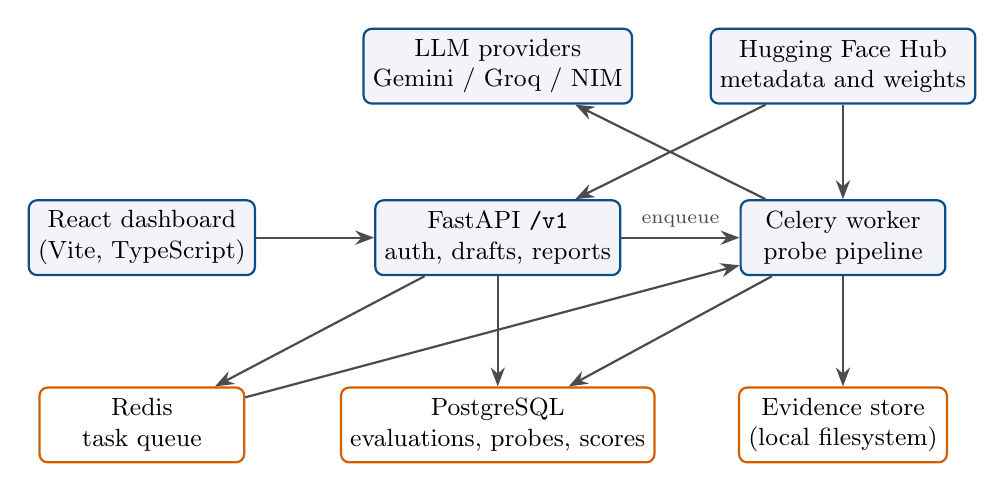
\begin{tikzpicture}[font=\small,
  box/.style={draw=tlblue,fill=tlgrey,rounded corners=3pt,minimum height=0.95cm,minimum width=2.6cm,align=center,thick},
  store/.style={draw=tlorange,fill=white,rounded corners=3pt,minimum height=0.95cm,minimum width=2.6cm,align=center,thick},
  arr/.style={-{Stealth[length=2.4mm]},thick,color=black!70}]
  \node[box] (ui) {React dashboard\\(Vite, TypeScript)};
  \node[box,right=1.5cm of ui] (api) {FastAPI \code{/v1}\\auth, drafts, reports};
  \node[box,right=1.5cm of api] (wk) {Celery worker\\probe pipeline};
  \node[store,below=1.4cm of api] (pg) {PostgreSQL\\evaluations, probes, scores};
  \node[store,below=1.4cm of wk] (fs) {Evidence store\\(local filesystem)};
  \node[store,below=1.4cm of ui] (rd) {Redis\\task queue};
  \node[box,above=1.2cm of wk] (hf) {Hugging Face Hub\\metadata and weights};
  \node[box,above=1.2cm of api] (llm) {LLM providers\\Gemini / Groq / NIM};
  \draw[arr] (ui) -- (api);
  \draw[arr] (api) -- (wk) node[midway,above,font=\scriptsize]{enqueue};
  \draw[arr] (api) -- (pg);
  \draw[arr] (wk) -- (pg);
  \draw[arr] (wk) -- (fs);
  \draw[arr] (api) -- (rd);
  \draw[arr] (rd) -- (wk);
  \draw[arr] (hf) -- (wk);
  \draw[arr] (hf) -- (api);
  \draw[arr] (wk) -- (llm);
\end{tikzpicture}
\caption{Deployment architecture of TrustLens.}\label{fig:arch}
\end{figure}

The API process validates requests, stores model records and evaluation drafts, and enqueues a Celery task \code{trustlens.evaluate\_model}. The worker loads the model through the inference backend, runs the probes, stores raw evidence, asks the O/S/D engine for ratings, calls the scorer, and writes everything back to PostgreSQL. The browser then reads the finished evaluation and its report.

\section{Component view}
Figure~\ref{fig:components} groups the Python packages under \code{backend/app} by responsibility.

\begin{figure}[H]
\centering
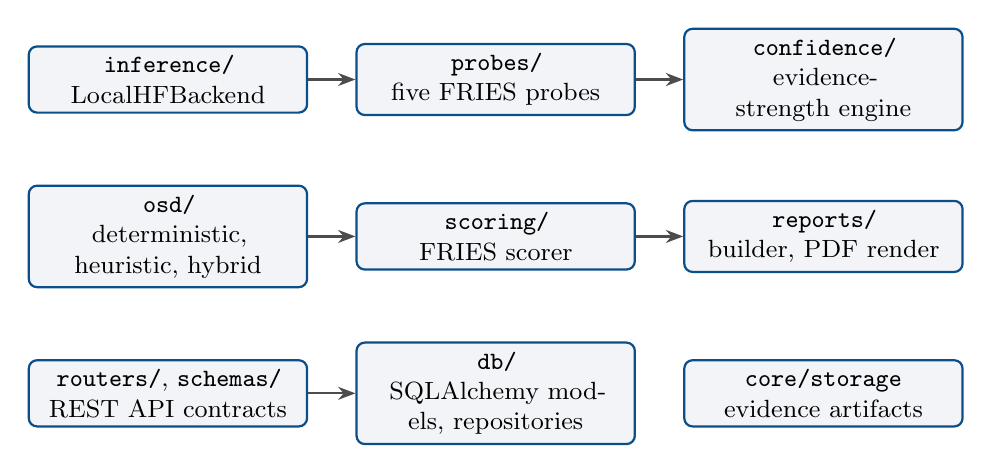
\begin{tikzpicture}[font=\small,
  c/.style={draw=tlblue,fill=tlgrey,rounded corners=3pt,minimum height=0.8cm,text width=3.3cm,align=center,thick},
  g/.style={draw=tlrule,dashed,rounded corners=4pt,inner sep=7pt},
  arr/.style={-{Stealth[length=2.2mm]},thick,color=black!70}]
  \node[c] (inf) {\code{inference/}\\LocalHFBackend};
  \node[c,right=0.6cm of inf] (prb) {\code{probes/}\\five FRIES probes};
  \node[c,right=0.6cm of prb] (cnf) {\code{confidence/}\\evidence-strength engine};
  \node[c,below=0.9cm of inf] (osd) {\code{osd/}\\deterministic, heuristic, hybrid};
  \node[c,right=0.6cm of osd] (sc) {\code{scoring/}\\FRIES scorer};
  \node[c,right=0.6cm of sc] (rep) {\code{reports/}\\builder, PDF render};
  \node[c,below=0.9cm of osd] (api) {\code{routers/}, \code{schemas/}\\REST API contracts};
  \node[c,right=0.6cm of api] (db) {\code{db/}\\SQLAlchemy models, repositories};
  \node[c,right=0.6cm of db] (st) {\code{core/storage}\\evidence artifacts};
  \draw[arr] (inf) -- (prb); \draw[arr] (prb) -- (cnf);
  \draw[arr] (osd) -- (sc); \draw[arr] (sc) -- (rep);
  \draw[arr] (api) -- (db); 
\end{tikzpicture}
\caption{Main packages of the backend and their dependencies.}\label{fig:components}
\end{figure}

\section{Execution flow of an audit}
Figure~\ref{fig:seq} shows the sequence of one evaluation as the code performs it. The probe order in the runner is Fairness, Robustness, Integrity, Explainability, Safety.

\begin{figure}[H]
\centering
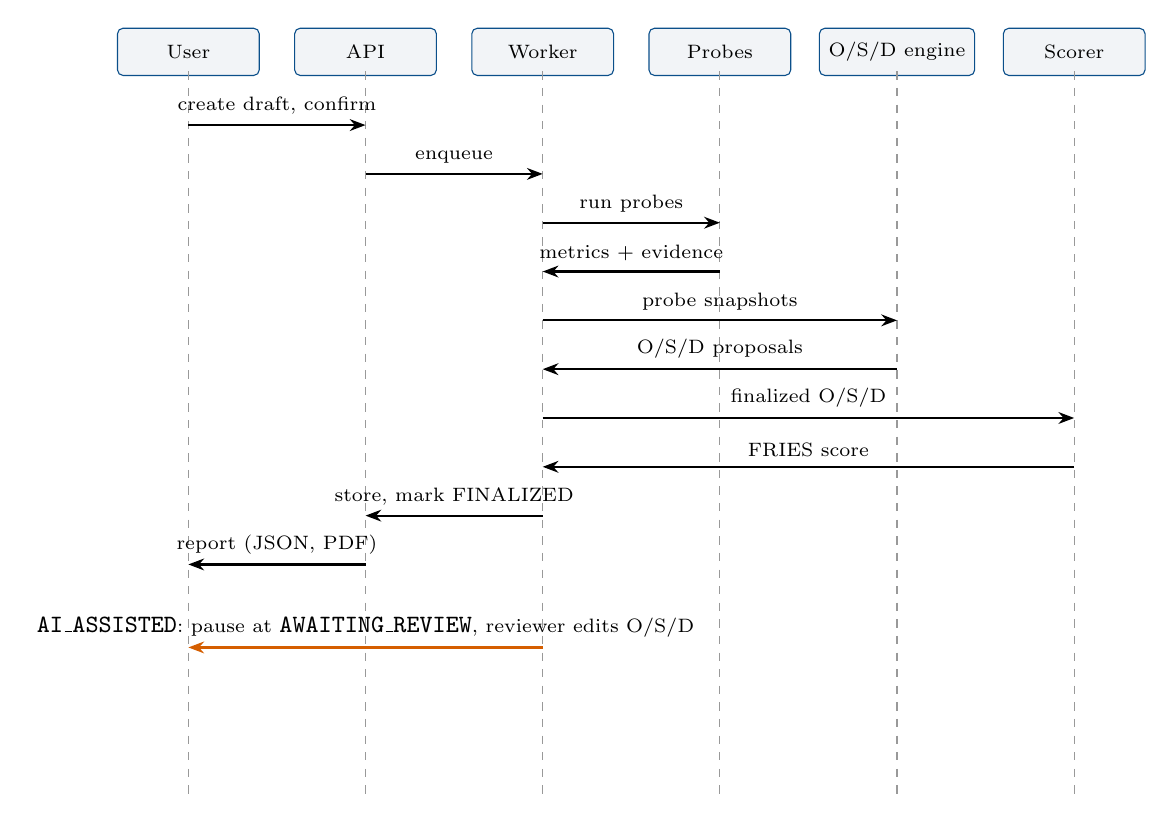
\begin{tikzpicture}[font=\scriptsize,x=2.25cm,y=-0.62cm,
  life/.style={dashed,color=black!40},
  m/.style={-{Stealth[length=2mm]},thick}]
  \foreach \i/\n in {0/User,1/API,2/Worker,3/Probes,4/{O/S/D engine},5/Scorer} {
    \node[draw=tlblue,fill=tlgrey,rounded corners=2pt,minimum width=1.8cm,minimum height=0.6cm] (n\i) at (\i,0) {\n};
    \draw[life] (\i,0.4) -- (\i,15.2);
  }
  \draw[m] (0,1.5) -- (1,1.5) node[midway,above]{create draft, confirm};
  \draw[m] (1,2.5) -- (2,2.5) node[midway,above]{enqueue};
  \draw[m] (2,3.5) -- (3,3.5) node[midway,above]{run probes};
  \draw[m] (3,4.5) -- (2,4.5) node[midway,above]{metrics + evidence};
  \draw[m] (2,5.5) -- (4,5.5) node[midway,above]{probe snapshots};
  \draw[m] (4,6.5) -- (2,6.5) node[midway,above]{O/S/D proposals};
  \draw[m] (2,7.5) -- (5,7.5) node[midway,above]{finalized O/S/D};
  \draw[m] (5,8.5) -- (2,8.5) node[midway,above]{FRIES score};
  \draw[m] (2,9.5) -- (1,9.5) node[midway,above]{store, mark FINALIZED};
  \draw[m] (1,10.5) -- (0,10.5) node[midway,above]{report (JSON, PDF)};
  \draw[m,color=tlorange] (2,12.2) -- (0,12.2) node[midway,above,color=black]{\code{AI\_ASSISTED}: pause at \code{AWAITING\_REVIEW}, reviewer edits O/S/D};
\end{tikzpicture}
\caption{Sequence of a TrustLens evaluation.}\label{fig:seq}
\end{figure}

\section{Data flow and evaluation contract}
Each evaluation carries an \emph{evaluation contract} (schema \code{v2} in \code{schemas/evaluation\_contract\_v2.py}) that makes the evaluation explicit rather than implicit. For Fairness and Robustness it records: the content-addressed dataset (\code{dataset\_content\_id}), the text and target columns, the sensitive-attribute column, a \code{label\_mapping} from dataset values to model label indices, \code{min\_group\_n}, and the \code{positive\_label\_index} that demographic parity treats as the favourable outcome. It also freezes a \code{model\_label\_snapshot} (the model's \code{id2label}) and the resolved model revision. We found this contract design valuable during the experiment, because it made the label mapping problem described in Chapter~\ref{ch:results} visible after the fact: the snapshot of \code{unitary/toxic-bert} lists six labels, and the mapping sends dataset value~1 to index~1, which is \code{severe\_toxic}.

\begin{figure}[H]
\centering
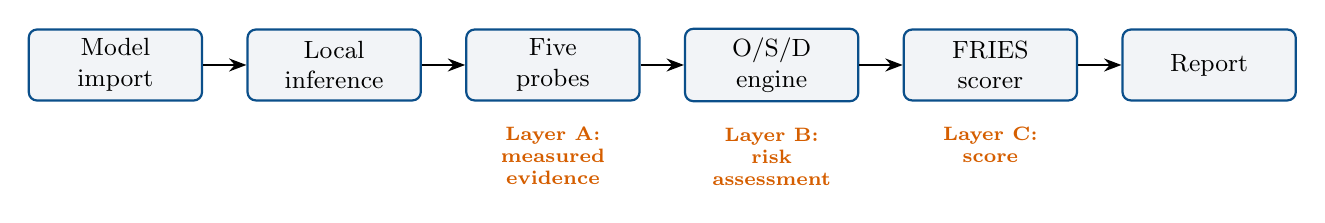
\begin{tikzpicture}[font=\small,node distance=0.55cm,
  p/.style={draw=tlblue,fill=tlgrey,rounded corners=3pt,minimum height=0.9cm,minimum width=2.2cm,align=center,thick},
  l/.style={font=\scriptsize\bfseries,color=tlorange},
  arr/.style={-{Stealth[length=2.2mm]},thick}]
  \node[p] (a) {Model\\import};
  \node[p,right=of a] (b) {Local\\inference};
  \node[p,right=of b] (c) {Five\\probes};
  \node[p,right=of c] (d) {O/S/D\\engine};
  \node[p,right=of d] (e) {FRIES\\scorer};
  \node[p,right=of e] (f) {Report};
  \foreach \x/\y in {a/b,b/c,c/d,d/e,e/f} \draw[arr] (\x) -- (\y);
  \node[l,below=0.2cm of c,align=center] {Layer A:\\measured\\evidence};
  \node[l,below=0.2cm of d,align=center] {Layer B:\\risk\\assessment};
  \node[l,below=0.2cm of e,align=center] {Layer C:\\score};
\end{tikzpicture}
\caption{Execution pipeline and the three evidence layers. Layer~A outputs are never turned directly into a dimension score.}\label{fig:pipeline}
\end{figure}

\section{Evaluation modes and assessment engines}
Two orthogonal switches control an evaluation.

\textbf{Workflow mode.} \code{AI\_AUTONOMOUS} lets the pipeline finalise without a reviewer (the report is marked \code{human\_reviewed=false}); \code{AI\_ASSISTED} stops so a reviewer can edit O/S/D. Despite the enum names, no language model is involved in the mode itself; they are human-review gates.

\textbf{Assessment engine.} \code{deterministic} (default) never proposes O/S/D and therefore withholds the FRIES score; \code{legacy\_heuristic} maps probe metrics to bands with fixed rules; \code{llm\_v1} starts from the heuristic output and then asks an LLM to re-rate Integrity, Explainability and Safety. Fairness and Robustness always keep the heuristic ratings computed from measured metrics. The experiments in this report use \code{llm\_v1} in \code{AI\_AUTONOMOUS} mode, which is why a repeated run can produce different numbers (Section~\ref{sec:variance}).

\chapter{The FRIES Framework in TrustLens}\label{ch:fries}

\section{From evidence to score}
FRIES, as proposed by Rutinowski et~al.\ \cite{rutinowski2024}, adapts FMEA to trust. For each relevant risk an analyst rates \emph{Occurrence} (O), \emph{Severity} (S) and \emph{Detection} (D), and the ratings are combined into a score. TrustLens uses the convention that \textbf{higher is better on all three scales}: a high O means the failure is unlikely, a high S means the consequence is mild, and a high D means the failure is easy to detect. Mixing this up with ordinary FMEA, where high means dangerous, would invert the result, so the scorer validates that all three values are integers in $0..10$.

The arithmetic in \code{scoring/fries.py} is short enough to state completely:
\begin{align}
\Pi_r &= \sqrt[3]{O_r\, S_r\, D_r}, \qquad \Pi_r = 0 \text{ if any of } O_r,S_r,D_r = 0 \text{ (veto)},\\
T_a &= \frac{1}{|R_a|}\sum_{r\in R_a}\Pi_r, \qquad
\text{FRIES} = \sum_{a} w_a\, T_a, \quad w_a = 0.2 \text{ by default.}
\end{align}
Custom weights must each be at least $0.1$ and sum to one. In every experiment of this report there is one risk per dimension, so $T_a=\Pi_r$, and the weights are equal.

The geometric mean has a consequence worth stating: a single very low component pulls the risk score down much more than an arithmetic mean would. For example, $(O,S,D)=(1,2,2)$ gives $\Pi=\sqrt[3]{4}=1.59$, whereas $(9,9,8)$ gives $8.65$. This is why documentation-poor models fall so far in our results.

\paragraph{Three layers.} TrustLens separates (A) \emph{measured evidence} such as a parity gap or a hash, (B) \emph{risk assessment}, the O/S/D proposal, and (C) the score. The README states that a raw metric must never be treated as a dimension score. The implemented heuristic engine does come close to violating this rule, because its bands are simple functions of one metric (for instance Fairness O is a function of the parity gap alone). The README lists this under known methodological gaps, and we repeat it here because it affects how the results should be read.

\section{Probes at a glance}
\begin{table}[H]
\centering\footnotesize
\caption{How each FRIES dimension is operationalised in the implemented code.}\label{tab:probes}
\begin{tabularx}{\textwidth}{@{}p{1.9cm}LLL@{}}
\toprule
\textbf{Dimension} & \textbf{Input} & \textbf{Evidence produced} & \textbf{Runs the model?}\\
\midrule
Fairness & Labelled CSV with a sensitive-attribute column; label mapping & DPD, EOD, subgroup-F1 spread, bootstrap 95\% CIs, group sizes & Yes (user-defined local mode); proxy logistic regression on Adult in the older mode\\
Robustness & Labelled text samples & Clean accuracy, accuracy after character swaps, accuracy drop with paired bootstrap CI, Wilson intervals & Yes (text classification only)\\
Integrity & Hub metadata of the model & Six metadata checks, named risks \code{I-INT-*}, hash gates & No (metadata); hash comparison only if two hashes are supplied\\
Explainability & Model card text & Presence of five required sections, contradiction flags & No (card only)\\
Safety & Model card text & Presence of four disclosure items, high-impact-claim flags & No (card only)\\
\bottomrule
\end{tabularx}
\end{table}

\section{Fairness}
\textbf{Definition and purpose.} A model is group-fair, in the sense measured here, when its behaviour does not differ much across groups defined by a sensitive attribute. It matters for toxicity moderation in particular, since an over-flagging model silences some speakers.

\textbf{Implementation.} \code{fairness\_metrics.py} computes, with binary positive class $\hat y = $\code{positive\_label\_index}:
\begin{itemize}
\item $\mathrm{DPD} = \max_g P(\hat Y{=}1\mid g)-\min_g P(\hat Y{=}1\mid g)$,
\item $\mathrm{EOD} = \max(\Delta\mathrm{TPR},\Delta\mathrm{FPR})$ across groups,
\item subgroup F1 spread $= \max_g F1_g - \min_g F1_g$.
\end{itemize}
Groups smaller than \code{min\_group\_n} (30 in our runs) are excluded, and \code{fairness\_stats.py} adds a percentile bootstrap CI ($B=1000$). Predictions come from the local inference backend running the imported model.

\textbf{Mapping to O/S/D (heuristic).} Let $\text{gap}=\max(|\mathrm{DPD}|,|\mathrm{EOD}|)$. Then $O=S=\mathrm{clip}_{1..9}(\mathrm{round}(10(1-\text{gap})))$ and $D=8$ (7 if a group is thin). For the label-flipped model V1, gap $=0.418$ gives $(6,6,8)$.

\textbf{Interpretation and limits.} DPD compares raw positive rates, so it also reports differences that come from real base-rate differences between groups. A model that is perfectly accurate on a dataset where one group contains more toxic comments will show a nonzero DPD. The EOD and F1-spread are less affected, but all three depend on a single sensitive attribute (here a binary ``identity mentioned'' flag).

\section{Robustness}
\textbf{Implementation.} \code{robustness\_nlp.py} replaces up to \code{max\_changes}$=3$ alphanumeric characters per text with random lowercase letters or digits (seeded RNG), runs both the clean and the perturbed text through the model, and \code{robustness\_eval.py} computes clean accuracy, robust accuracy and the paired accuracy drop with a bootstrap CI. A named risk \code{R-ROB-PERT} fires when the drop exceeds $\varepsilon=0.05$ at 95\% confidence. Gates reject the run if fewer than 100 samples were evaluated, if fewer than 95\% of samples are label-compatible, or if clean accuracy is below 0.20.

\textbf{Mapping to O/S/D.} The heuristic engine sets $O=\mathrm{scale}(\text{clean acc.})$, $S=\mathrm{scale}(\text{robust acc.})$ and $D=\mathrm{scale}(\min(\text{robust}/\text{clean},1))$. Two things follow, and both matter later. First, the band is dominated by raw accuracy, so a mediocre but stable model scores low. Second, a 4-point accuracy drop changes the ratio from 1.00 to about 0.95, and after rounding the band moves by at most one step.

\textbf{Limits.} Random character swaps are a weak attack. They test sensitivity to typos, not adversarial robustness; a gradient-guided attack \cite{ebrahimi2018} would be stronger. Models whose output collapses to one class are trivially stable under any perturbation, a failure mode we ran into when designing the robustness-flawed variant (Section~\ref{sec:variants}).

\section{Integrity}
\textbf{Implementation.} \code{integrity\_eval.py} (\code{tl-integrity-v1.0}) works on Hub metadata. It checks whether a card is present, whether the file list is available, whether the revision is pinned to a commit hash, whether a licence is declared, whether the file listing was recorded, and whether the card makes reproducibility claims (training data, seed, evaluation, hyperparameters). Named risks include \code{I-INT-REV-UNPINNED}, \code{I-INT-MANIFEST-MISSING}, \code{I-INT-LICENSE-UNDISCLOSED}, \code{I-INT-BYTES-DIVERGE} and \code{I-INT-LISTING-DRIFT}. Hash verification requires both a trusted reference hash and a local artifact hash; when either is missing the probe records the gates \code{G-INT-HASH-REF-MISSING} and \code{G-INT-HASH-LOCAL-MISSING} and states that cryptographic identity was \emph{not} verified.

\textbf{Limits.} The probe documents identity and disclosure. It does not detect tampered weights unless a trusted reference hash is supplied, and in none of our runs was one supplied. The code's own limitation text says so: integrity risks ``measure disclosure and identity recording, not tampering or legal compliance''.

\section{Explainability}
\textbf{Implementation.} In TrustLens, explainability means transparency of documentation. \code{explainability\_card.py} searches the card for five required sections (intended use, limitations, training data, evaluation, ethical considerations; bonus sections are tracked separately), and the coverage ratio is the number of required sections present divided by five. \code{explainability\_eval.py} also flags contradictions such as \code{open\_claim\_vs\_restrictive\_license} and \code{no\_limitations\_but\_production\_claim}. Template placeholders such as ``[More Information Needed]'' are rejected by \code{card\_markdown.nontrivial()}.

\textbf{Limits.} This is not SHAP or LIME and says nothing about whether a human can understand \emph{why} the model made a prediction. It measures whether the author wrote the sections, and the heuristic reads headings, so a card with the right headings and empty content can pass the probe (the LLM step in \code{llm\_v1} is meant to catch this).

\section{Safety}
\textbf{Implementation.} \code{safety\_card.py} (\code{tl-safety-v1.0}) looks for four disclosure items: misuse risks, privacy, security warnings and data disclosure, and flags high-impact deployment claims (for example ``production ready for any use'') made without full disclosure.

\textbf{Limits.} There is no behavioural safety test set in the repository: nothing here feeds unsafe prompts to the model or checks how often it misses harmful content. The Safety score therefore describes the governance paperwork, not the model's behaviour. This limitation drives the main negative result of Chapter~\ref{ch:results}.

\section{O/S/D engines}
\begin{description}[leftmargin=1.2em]
\item[Deterministic] Abstains: all O, S, D are \code{None}, FRIES is withheld. Default, because the project has no validated metric-to-O/S/D mapping.
\item[Heuristic] The band rules above. For cards: $O=S=D=\mathrm{scale}(\text{coverage})$, with $S{-}2$ and $D{-}1$ when high-impact claims have gaps; an empty card gets the fixed band $(2,2,3)$. Integrity: $O=S=\mathrm{scale}(\text{pass rate})$, $D=8$.
\item[LLM-assisted (\code{llm\_v1})] One batched prompt asks a hosted model (Gemini first, then Groq, then NVIDIA NIM, in that order of preference) to give O, S, D from 1 to 9 for Integrity, Explainability and Safety, using the quoted card text and the probe evidence, with a 3--5 sentence rationale. If every provider fails, the heuristic values are kept and tagged \code{heuristic\_fallback}. All three are labelled ``proposed, not ground truth'' in the report.
\end{description}

\chapter{Implementation Details}\label{ch:impl}

\section{Technology stack}
Table~\ref{tab:stack} lists the technologies that the code actually imports. Libraries that only appear in dependency files are not listed.

\begin{table}[H]
\centering\small
\caption{Technology stack and role of each component.}\label{tab:stack}
\begin{tabularx}{\textwidth}{@{}p{3.2cm}L@{}}
\toprule
\textbf{Technology} & \textbf{Role in TrustLens}\\
\midrule
Python $\ge$3.11 & Backend, worker, probes, experiment scripts.\\
FastAPI, Pydantic v2 & REST API under \code{/v1}; Pydantic models define the evaluation contract, probe output and report schemas.\\
SQLAlchemy 2, Alembic, PostgreSQL & Persistence; fourteen migrations track the schema (e.g.\ dataset content, draft state, methodology version).\\
Celery, Redis & Asynchronous execution of the evaluation pipeline in a worker process.\\
Hugging Face \code{transformers} \cite{wolf2020}, PyTorch & Local inference in \code{LocalHFBackend}; \code{AutoConfig} for cheap model inspection.\\
\code{huggingface\_hub} & Metadata import (card, tags, licence, file list).\\
\code{google-genai}, \code{httpx} & LLM calls to Gemini, Groq and NVIDIA NIM for the \code{llm\_v1} engine.\\
Jinja2, WeasyPrint & HTML report template rendered to PDF.\\
React 19, Vite, TypeScript, React Router & Dashboard: model import, draft wizard, evaluation timeline, review and report pages.\\
Vitest, pytest, ruff & Frontend tests, backend tests, linting (also run in GitHub Actions).\\
Docker Compose & Five services: postgres, redis, api, worker, frontend; separate CPU-only and GPU compose files.\\
\bottomrule
\end{tabularx}
\end{table}
The GPU-related choices follow from the reference machine described in the specification: an RTX 4060 Laptop GPU with 8~GB of VRAM. Our experiment logs confirm CUDA execution with float32 weights and batch size~8 (\code{execution\_metadata}).

\section{Important modules}
\begin{table}[H]
\centering\small
\caption{Key source files and responsibilities.}
\begin{tabularx}{\textwidth}{@{}p{4.3cm}L@{}}
\toprule
\textbf{File} & \textbf{Purpose, inputs and outputs}\\
\midrule
\code{inference/local\_hf.py} & Loads a sequence-classification model and tokenizer, batches texts, applies softmax, returns predictions plus device metadata. Raises typed errors on load or inference failure.\\
\code{inference/device.py} & Chooses CUDA or CPU and records the reason (\code{device\_reason}) and any fallback.\\
\code{probes/runner.py} & Runs probes in order, validates each output (dimension match, confidence in $[0,1]$, evidence present), persists \code{probe\_results} and refines confidence.\\
\code{probes/fairness.py}, \code{fairness\_metrics.py}, \code{fairness\_stats.py} & Subgroup predictions, DPD/EOD/F1 spread, bootstrap CI.\\
\code{probes/robustness\_nlp.py}, \code{robustness\_eval.py} & Char-swap attack and accuracy-drop evaluation with gates.\\
\code{probes/integrity\_eval.py}, \code{explainability\_eval.py}, \code{safety\_eval.py} & Pure functions over Hub metadata and card text.\\
\code{confidence/engine.py} & Evidence-strength score: geometric mean of data quality, probe reliability and evidence completeness. Marked uncalibrated.\\
\code{osd/agent.py}, \code{hybrid.py}, \code{llm\_client.py} & Heuristic bands; LLM prompt, call, parse, fallback.\\
\code{scoring/fries.py} & Cube-root risk score, veto, aspect mean, weighted total.\\
\code{reports/builder.py} & Builds the canonical \code{report\_v1} JSON; PDF is a projection of it. Append-only versions.\\
\bottomrule
\end{tabularx}
\end{table}

\paragraph{Evidence and reproducibility features.} Each probe stores its raw output as a JSON artifact with a SHA-256 hash; evaluations are stamped with an immutable \code{methodology\_version}; model revisions are frozen at draft time and the loaded snapshot is verified against it (\code{model\_snapshot\_check.py}); and probes take an explicit seed. Our determinism check is in Section~\ref{sec:determinism}.

\paragraph{Documentation discrepancy.} The project README still lists JWT roles (researcher, reviewer, admin) among the working features, and the setup script prints a \code{seed\_users} step. The code does not match: migration \code{008\_remove\_auth\_and\_ownership} removed authentication and ownership, and there is no \code{seed\_users} module under \code{backend/app/scripts}. We follow the code, and we omit that step from the commands below.

\paragraph{Error handling.} Probe outputs that violate the contract raise \code{ProbeError} and fail the evaluation rather than being stored. A probe that cannot run records a status (\code{INSUFFICIENT\_EVIDENCE}, \code{SKIPPED}, \code{NOT\_APPLICABLE}, \code{FAILED} or \code{PROXY}) instead of a number. The API returns a conflict (HTTP 409) for a report on an evaluation whose FRIES score was withheld, rather than pretending the report is merely not ready.

\section{Installation and execution}
The following commands are taken from the repository (\code{docs/TRUSTLENS\_LOCAL\_DEVELOPMENT.md}, \code{scripts/}, \code{Makefile}). Prerequisites: Python 3.11+, Node 18+, Docker Desktop with Compose v2; an NVIDIA GPU is optional but used when present.

\begin{lstlisting}
# one-time backend setup (Windows PowerShell)
.\scripts\setup-local-dev.ps1
.\.venv\Scripts\Activate.ps1
docker compose up -d postgres redis
cd backend; alembic upgrade head
uvicorn app.main:app --reload --host 127.0.0.1 --port 8000
# in other terminals: worker and frontend
.\scripts\dev-worker.ps1      # Celery worker
.\scripts\dev-frontend.ps1    # React dashboard (npm run dev)
# tests
cd backend; python -m pytest -q
\end{lstlisting}

To reproduce the forged-model experiment (docstrings of the three scripts under \code{backend/app/scripts}, run from \code{backend/}):
\begin{lstlisting}
python -m app.scripts.prepare_flawed_suite_data      # builds eval_set + per-variant train slices
python -m app.scripts.train_flawed_suite --all       # fine-tunes variants 1,2,3,5,6
python -m app.scripts.run_flawed_suite_eval          # evaluates all 7 models through the API
\end{lstlisting}
The last script needs the Compose stack running and the local model directory bind-mounted into the worker at \code{/models/flawed\_model\_suite}. Output is written to \code{results/flawed\_model\_suite/}. A user normally interacts through the dashboard: import a model, create an evaluation draft, attach a dataset and label mapping, confirm, and read the report. In the report, the FRIES score is shown next to the evidence, the O/S/D ratings with their rationale, the evidence-strength confidence, and a disclosure that states the mode, the engine and whether a human reviewed the numbers.

\chapter{Experimental Design}\label{ch:experiment}

\section{Question and hypothesis}
The research question for the experiment is RQ2 from Chapter~\ref{ch:intro}: \emph{can TrustLens distinguish a reference model from models that we deliberately made worse?}

We state the hypothesis in a form that can fail:

\begin{quote}
\textbf{H1.} If the FRIES probes capture trust-relevant properties, then a forged model should obtain a \emph{lower score on the FRIES dimension in which its flaw was injected} than the reference model does, and a model carrying flaws in several dimensions should obtain the lowest overall score.
\end{quote}
We also record a weaker, secondary hypothesis, \textbf{H2}: the overall FRIES score of each forged model is lower than that of the reference. We expected H2 to be harder to satisfy, because an overall score averages over four dimensions that were left untouched. We wrote H1 and H2 before looking at the second run, but we had already seen the first run, so neither is a fully pre-registered prediction.

\section{Models}
\subsection{Model A: reference model}
\begin{table}[H]
\centering\small
\caption{Reference model.}
\begin{tabularx}{\textwidth}{@{}p{3.8cm}L@{}}
\toprule
Model & \code{unitary/toxic-bert} (Hugging Face Hub), the Detoxify BERT-based multi-label toxic comment classifier\\
Revision & \code{4d6c22e74ba2fdd26bc4f7238f50766b045a0d94} (pinned in the evaluation contract)\\
Architecture & BERT sequence classifier with six output labels: \code{toxic}, \code{severe\_toxic}, \code{obscene}, \code{threat}, \code{insult}, \code{identity\_hate}\\
Parameter count & \todo{read from model files; not recorded in the result JSON}\\
Training data, licence & As stated on the Hub card; our probes record that the card lacks explicit intended-use and training-data sections (coverage 0.6)\\
Conversion for evaluation & TrustLens decides with argmax over a softmax, which cannot express ``toxic versus not toxic'' on a six-way sigmoid head. We therefore built \code{reference\_toxicbert\_2label} (\code{convert\_reference\_2label.py}): encoder weights unchanged; new head with logit$_0=0$ and logit$_1$ equal to the original \code{toxic} logit, so $P_1=\sigma(z_{\text{toxic}})$ and argmax picks ``toxic'' exactly when the original output exceeds 0.5. A check on four sentences gave a maximum probability difference of $9.5{\times}10^{-4}$, so predictions very close to the boundary could differ from the original model.\\
Selection reason & Widely used, public, same task as our variants. \emph{It is not a certified trustworthy model}; we call it the reference model because it is an established public release, not because we have proof of its quality.\\
\bottomrule
\end{tabularx}
\end{table}

\subsection{Model B: forged variants}\label{sec:variants}
We could not obtain a real malicious model, so we built six. All start from \code{bert-base-uncased} \cite{devlin2019} and are fine-tuned for binary toxicity classification on a sample of Civil Comments \cite{borkan2019}; each variant's flaw was chosen to target one FRIES dimension, and the flip logic is recorded in a data manifest next to the weights. Table~\ref{tab:variants} summarises them.

\begin{table}[H]
\centering\footnotesize
\caption{The six forged variants. All use \code{bert-base-uncased}, seed 42, max sequence length 128. ``Rows'' is the training set size.}\label{tab:variants}
\begin{tabularx}{\textwidth}{@{}p{1.6cm}p{1.9cm}Lp{2.7cm}@{}}
\toprule
\textbf{Variant} & \textbf{Target} & \textbf{Injected flaw} & \textbf{Training}\\
\midrule
V1 & Fairness & 40\% of non-toxic comments that mention an identity (any annotator flagged an identity attack) had their label flipped to toxic: 249 of 8\,000 rows. Card is complete and honest about the flaw. & 3 epochs, lr $2{\times}10^{-5}$, wd 0.01, 8\,000 rows\\
V2 & Robustness & Class-balanced narrow training set (all 628 toxic rows plus 628 non-toxic), 4 epochs, lr $5{\times}10^{-5}$, no weight decay, intended to produce a brittle model. Redesigned after a first design collapsed to a majority-class predictor. & 4 epochs, 1\,256 rows\\
V3 & Explainability & Weights trained on clean labels; the model card is the untouched auto-generated template (``[More Information Needed]'' everywhere). & 3 epochs, 8\,000 rows\\
V4 & Integrity & \emph{Weights are an exact copy of V1.} The card claims ``production ready'', ``no known biases'', ``no material risks'', declares licence \code{other} while claiming unrestricted commercial use, and omits the limitations. & none (copy of V1)\\
V5 & Safety & 50\% of rows with any severe-toxicity annotation relabelled as non-toxic (244 of 8\,000), so the model under-flags severe toxicity. Card is complete and honest. & 3 epochs, 8\,000 rows\\
V6 & Compound & V1 flip and V5 relabelling applied in sequence; template card with over-claiming sentence added; licence \code{other}. & 3 epochs, 8\,000 rows\\
\bottomrule
\end{tabularx}
\end{table}
Each fine-tuning took about 160 seconds on the RTX 4060 laptop GPU (V2, with fewer rows, is not timed in its manifest). Each resulting checkpoint is a float32 BERT-base model of 437.96\,MB (about 109.5 million parameters including the classification head).

\paragraph{What the forged models are, and are not.} They are experimental constructs for probing the tool. They do not represent real-world malicious models: nobody planted a backdoor, nothing adapts to the evaluator, and several flaws sit in the model card, which an attacker could trivially fix. Three of the six variants (V3, V4, V6) are essentially \emph{documentation} flaws wrapped around weights that behave like an ordinary fine-tuned BERT, and V4 is behaviourally identical to V1. This matters for what a ``detection'' means, and we come back to it in Chapter~\ref{ch:discussion}.

\paragraph{A design lesson.} Our first V2 used 600 rows and 12 epochs to overfit. Instead it collapsed to a majority-class predictor that predicted positive for only 0.6--8.4\% of inputs, which is more stable under perturbation than the reference, not less (accuracy drop 0.3--0.9 points). The manifest records this diagnosis. It taught us that a robustness probe built on accuracy drop cannot see a constant predictor as a problem, and the same issue appears again in the reference model (Section~\ref{sec:constant}).

\section{Variables and controls}
\begin{table}[H]
\centering\small
\caption{Experimental variables.}
\begin{tabularx}{\textwidth}{@{}p{3.6cm}L@{}}
\toprule
Independent variable & Which model is evaluated (reference or one of V1--V6): weights, model card and licence field.\\
Dependent variables & Per-probe measured evidence (DPD, EOD, F1 spread, clean and robust accuracy, card coverage, integrity risks); per-dimension scores; overall FRIES score.\\
Controlled & Evaluation dataset (3\,000 rows of the Civil Comments \code{test} split, seed 42, 20\% positive rate, identical for all seven models); sensitive attribute (binary \code{identity\_ref} flag); label mapping; \code{min\_group\_n}$=30$; probe seed 42; assessment engine \code{llm\_v1}; mode \code{AI\_AUTONOMOUS}; hardware (RTX 4060 Laptop, CUDA, float32, batch 8); software stack.\\
Not controlled & The LLM that rates Integrity, Explainability and Safety (provider and sampling are not pinned or logged in the result file); the Hub-versus-local difference in model identity (Section~\ref{sec:threats}); the architecture and label head of the reference model, which differ from the variants'.\\
\bottomrule
\end{tabularx}
\end{table}

\paragraph{Sensitive attribute.} \code{identity\_ref} is 1 when the Civil Comments row has \code{identity\_attack}$>0.0001$; group sizes in the evaluation set are 2\,461 (value 0) and 539 (value 1). The same threshold is used when the V1 and V6 flip was injected, so the fairness probe evaluates the very attribute that the flaw targets. We note this as a favourable design for detection.

\paragraph{Runs.} The full set of seven evaluations was executed twice. Run~1 was created between 20:49 and 20:57 UTC on 14 September 2026, with the redesigned V2 evaluated at 21:23. Run~2 was created between 23:57 UTC that day and 00:06 UTC on 15 September. The two runs are \emph{not} exact replicates: Run~2 records an extra integrity gate (\code{G-INT-LISTING-UNVERIFIED}) that Run~1 does not, so the integrity probe changed in between, and the LLM that rates three dimensions is stochastic. We therefore treat them as two independent measurements of a slightly evolving tool. \emph{Run~3} is a single evaluation of the converted reference model (\code{eval\_results\_v3}), made after we found the label-mapping problem described in Section~\ref{sec:constant}. It uses the same dataset, mapping, mode, engine and hardware as Runs~1 and~2. The original Hub import of \code{toxic-bert} is called the \emph{original reference} below; the converted copy is the \emph{corrected reference}. Because the corrected reference is a local directory, the integrity probe treats it like the variants (no pinned revision, no file manifest), which makes its Integrity score comparable to theirs but not to the original reference's. Run~1 also contains an earlier V2 evaluation of the first (collapsed) V2 design, which we exclude from the tables; it remains in the repository. All figures and tables below are computed from the saved JSON files by \code{report/make\_figures.py}.

\section{Outcome measures}
For each model we report the five dimension scores and the overall FRIES score as produced by the tool, and the underlying evidence. For H1 we compare the \emph{targeted} dimension of each variant with the same dimension of the reference model. For H2 we compare overall scores. Because the sample is seven models, we use counts and plain differences, and we do not report significance tests.

\chapter{Results}\label{ch:results}

All numbers in this chapter come from the saved evaluation JSON files in \code{results/flawed\_model\_suite/eval\_results} (Run~1) and \code{eval\_results\_v2} (Run~2). ``G'' in tables is the \emph{original} reference (Hub import, six-label head, wrong label mapping); ``R*'' is the \emph{corrected} reference (Run~3), the one we use for hypothesis testing. Each evaluation reached status \code{FINALIZED} with five evaluated probes and no failures.

\section{Overall and per-dimension scores}
\begin{table}[H]
\centering\small
\caption{FRIES scores, Run~2. The flawed dimension of each variant is in bold. Scores are on a 0--10 scale; higher is better.}\label{tab:run2}
\begin{tabularx}{\textwidth}{@{}p{3.8cm}RRRRRR@{}}
\toprule
\textbf{Model} & \textbf{Fair.} & \textbf{Rob.} & \textbf{Integ.} & \textbf{Expl.} & \textbf{Safety} & \textbf{FRIES}\\
\midrule
G: toxic-bert (reference) & 8.65 & 8.32 & 5.01 & 3.63 & 1.59 & \textbf{5.44}\\
\midrule
V1 fairness & \textbf{6.60} & 9.00 & 3.91 & 9.00 & 3.91 & 6.49\\
V2 robustness & 5.85 & \textbf{8.32} & 4.64 & 8.00 & 4.38 & 6.24\\
V3 explainability & 7.32 & 9.00 & 1.82 & \textbf{1.82} & 1.82 & 4.35\\
V4 integrity & 6.60 & 9.00 & \textbf{3.30} & 2.62 & 2.29 & 4.76\\
V5 safety & 8.00 & 9.00 & 3.63 & 9.00 & \textbf{3.98} & 6.72\\
V6 compound (F+S, card) & 6.60 & 9.00 & 2.29 & 1.26 & \textbf{1.26} & 4.08\\
\bottomrule
\end{tabularx}
\end{table}

\begin{table}[H]
\centering\small
\caption{FRIES scores, Run~1 (V2 is the redesigned model used in both runs).}\label{tab:run1}
\begin{tabularx}{\textwidth}{@{}p{3.8cm}RRRRRR@{}}
\toprule
\textbf{Model} & \textbf{Fair.} & \textbf{Rob.} & \textbf{Integ.} & \textbf{Expl.} & \textbf{Safety} & \textbf{FRIES}\\
\midrule
G: toxic-bert (reference) & 8.65 & 8.32 & 7.32 & 6.00 & 3.63 & \textbf{6.79}\\
\midrule
V1 fairness & \textbf{6.60} & 9.00 & 4.31 & 8.32 & 4.58 & 6.56\\
V2 robustness & 5.85 & \textbf{8.32} & 4.00 & 8.65 & 2.88 & 5.94\\
V3 explainability & 7.32 & 9.00 & 1.00 & \textbf{1.00} & 1.00 & 3.86\\
V4 integrity & 6.60 & 9.00 & \textbf{2.00} & 2.29 & 1.59 & 4.30\\
V5 safety & 8.00 & 9.00 & 4.82 & 8.65 & \textbf{2.88} & 6.67\\
V6 compound & 6.60 & 9.00 & 2.62 & 1.59 & \textbf{1.59} & 4.28\\
\bottomrule
\end{tabularx}
\end{table}

\begin{figure}[H]
\centering
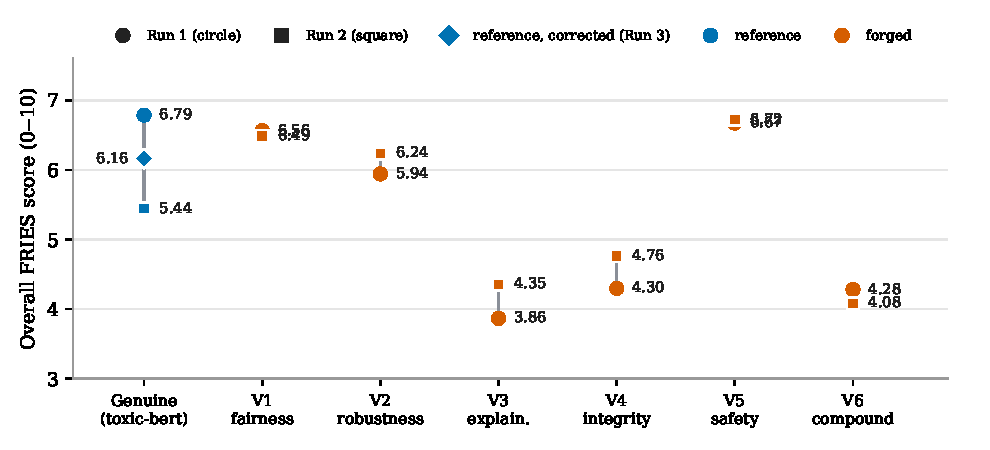
\includegraphics[width=0.92\textwidth]{fig_overall.pdf}
\caption{Overall FRIES score of every model in both runs. A vertical line joins the two runs of one model. The original reference moves the most between runs (1.34 points); the diamond is the corrected reference (Run~3).}\label{fig:overall}
\end{figure}

\begin{figure}[H]
\centering
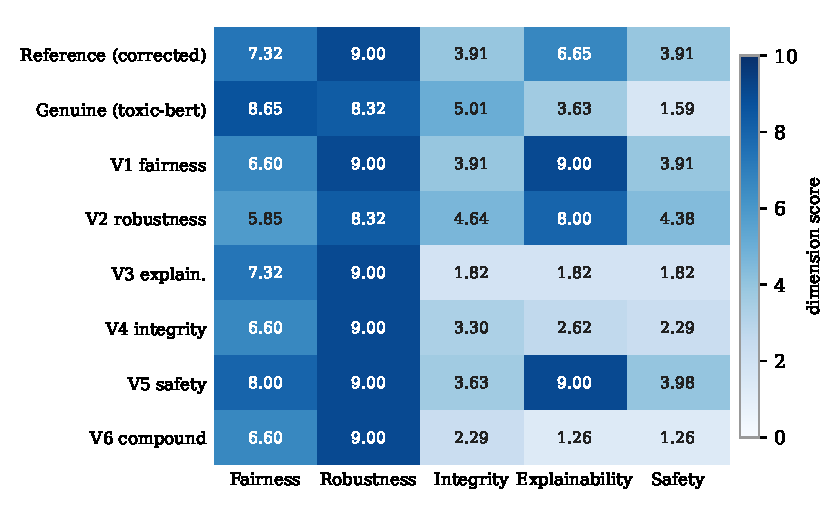
\includegraphics[width=0.78\textwidth]{fig_heatmap.pdf}
\caption{Dimension scores in Run~2; the first row is the corrected reference from Run~3. The columns that are uniformly dark for the variants with filled-in cards (Explainability, Safety) and the light rows for V3, V4 and V6 show where the score differences come from.}\label{fig:heatmap}
\end{figure}

\begin{figure}[H]
\centering
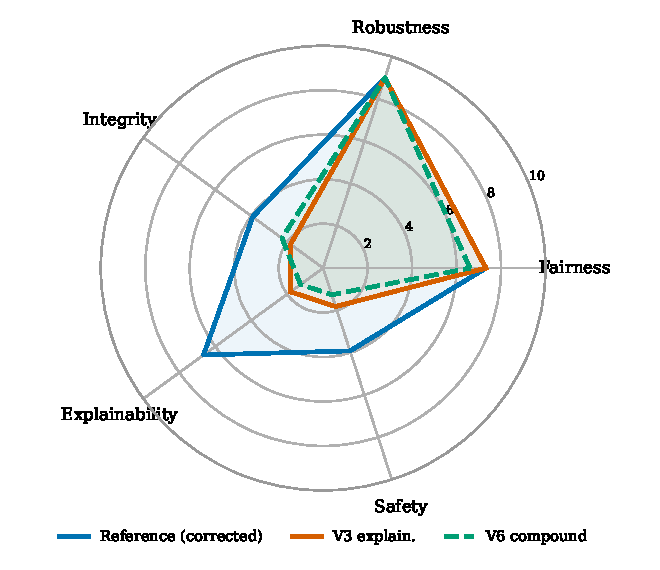
\includegraphics[width=0.62\textwidth]{fig_radar.pdf}
\caption{Run~2 FRIES profiles of V3 (blank card) and V6 (compound) against the corrected reference R* (Run~3). R* is weakest on Integrity and Safety, but V3 and V6 fall far below it on Explainability and Safety.}\label{fig:radar}
\end{figure}

\section{Measured evidence behind the scores}
Table~\ref{tab:evidence} lists what the probes actually measured in Run~2; the corrected reference follows in Table~\ref{tab:ref}. Fairness and Robustness were measured by running the model on the 3\,000 rows; the other three columns come from the card and metadata.

\begin{table}[H]
\centering\footnotesize
\caption{Measured evidence, Run~2. DPD with 95\% bootstrap CI; Drop is the char-swap accuracy drop in percentage points; Card cov.\ and Safety cov.\ are the fractions of required sections or checks found.}\label{tab:evidence}
\begin{tabularx}{\textwidth}{@{}p{0.8cm}p{3.5cm}RRRRRR@{}}
\toprule
 & \textbf{DPD [CI]} & \textbf{EOD} & \textbf{F1 spr.} & \textbf{Clean acc.} & \textbf{Drop} & \textbf{Card cov.} & \textbf{Safety cov.}\\
\midrule
G & 0.000 [0.000, 0.000] & 0.000 & 0.000 & 0.799 & $-$0.07 & 0.60 & 0.00\\
V1 & 0.418 [0.376, 0.464] & 0.164 & 0.123 & 0.897 & 1.47 & 1.00 & 0.25\\
V2 & 0.526 [0.487, 0.561] & 0.370 & 0.294 & 0.809 & 4.10 & 1.00 & 0.25\\
V3 & 0.319 [0.279, 0.363] & 0.065 & 0.074 & 0.894 & 1.17 & 0.60 & 0.25\\
V4 & 0.418 [0.376, 0.464] & 0.164 & 0.123 & 0.897 & 1.47 & 0.60 & 0.25\\
V5 & 0.233 [0.197, 0.275] & 0.035 & 0.033 & 0.876 & 1.30 & 1.00 & 0.25\\
V6 & 0.368 [0.327, 0.413] & 0.167 & 0.161 & 0.885 & 1.30 & 0.00 & 0.00\\
\bottomrule
\end{tabularx}
\end{table}

\begin{figure}[H]
\centering
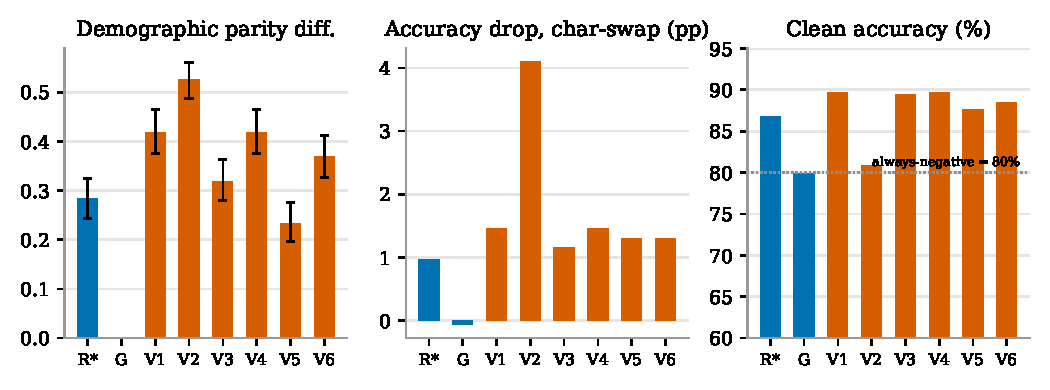
\includegraphics[width=\textwidth]{fig_probes.pdf}
\caption{Measured fairness and robustness evidence, Run~2. R* is the corrected reference (Run~3) and G the original one with the wrong label mapping. Left: demographic parity difference with bootstrap CI. Middle: accuracy drop under character swaps. Right: clean accuracy; the dotted line is the accuracy of a model that always answers ``not toxic'' on this sample.}\label{fig:probes}
\end{figure}

Three observations from Table~\ref{tab:evidence} and Figure~\ref{fig:probes} deserve attention.

\begin{itemize}
\item \textbf{V1 and V4 are identical in behaviour,} as they should be, since V4 reuses V1's weights. Every Fairness and Robustness metric, CI and O/S/D triple matches exactly. This is a useful sanity check that the behavioural probes are deterministic for fixed weights, data and seed.
\item \textbf{The fairness probe separated the flipped model from the clean model.} V1 has a DPD of 0.42 [0.38, 0.46]; V3, trained on the same data with no flip, has 0.32 [0.28, 0.36]. These intervals do not overlap. But V3's DPD is far from zero as well, and V5 and V6 show intermediate values, which is expected if part of the gap comes from the data and not from the injected flaw.
\item \textbf{The robustness flaw produced the largest accuracy drop (4.1 points), but the probe did not raise a risk.} The \code{R-ROB-PERT} trigger needs a drop of at least 5 points at 95\% confidence, and V2 sits below it. V2 also has the largest fairness gap (DPD 0.53), a side effect of its narrow training set that we did not design.
\end{itemize}

\section{The original reference was a constant predictor, and the corrected rerun}\label{sec:constant}
\subsection{Diagnosis}
The original reference model's demographic parity, equalized-odds and F1-spread are exactly zero, its clean accuracy is 0.7987, and the saved per-group statistics show a positive-prediction rate of 0.0 in \emph{both} identity groups: it never predicted ``toxic'' on this sample. Since 20\% of the sample is toxic, always answering ``not toxic'' would score 0.80, and the model scored 0.799. The cause is the label mapping. \code{unitary/toxic-bert} has six outputs, with \code{toxic} at index~0 and \code{severe\_toxic} at index~1, and our contract mapped dataset value~1 to index~1, so the probe checked whether \code{severe\_toxic} was the winning output. Its Fairness (8.65) and Robustness (8.32) scores in Tables~\ref{tab:run2} and~\ref{tab:run1} therefore say nothing about a working toxicity classifier: a constant predictor is trivially fair and trivially robust, and TrustLens raised no warning about it.

\subsection{Correction}
The tool offers no mapping that expresses ``toxic versus not toxic'' on this head: with argmax over six outputs a benign comment still selects some label, and no index stands for ``none''. We therefore converted the model to a two-label head with identical decision behaviour (Section~\ref{sec:variants} and Table~\ref{tab:ref}) and evaluated it through the unchanged pipeline, with the standard mapping (0$\to$0, 1$\to$1) and \code{positive\_label\_index}$=1$ (Run~3).

\begin{table}[H]
\centering\small
\caption{Corrected reference model (Run~3) against the original reference (Run~2).}\label{tab:ref}
\begin{tabularx}{\textwidth}{@{}p{4.1cm}RR@{}}
\toprule
 & \textbf{Original (G)} & \textbf{Corrected (R*)}\\
\midrule
Clean accuracy & 0.799 & 0.868\\
Positive-prediction rate, group 0 / group 1 & 0.000 / 0.000 & 0.051 / 0.334\\
DPD [95\% CI] & 0.000 [0.000, 0.000] & 0.283 [0.243, 0.324]\\
EOD / F1 spread & 0.000 / 0.000 & 0.174 / 0.203\\
Char-swap accuracy drop (pp) & $-$0.07 & 0.97\\
Fairness / Robustness score & 8.65 / 8.32 & 7.32 / 9.00\\
Integrity / Explainability / Safety & 5.01 / 3.63 / 1.59 & 3.91 / 6.65 / 3.91\\
Overall FRIES & 5.44 & 6.16\\
\bottomrule
\end{tabularx}
\end{table}
The corrected reference is a working classifier (86.8\% accuracy) and it, too, shows a demographic-parity gap of 0.28, because comments that mention identities are toxic more often in this dataset and the model reflects that. This is evidence that part of any DPD in this experiment is a base-rate effect and not a flaw, and it sets the fair comparison for V1: the label-flipped model's gap of 0.42 [0.38, 0.46] is clearly above the corrected reference's 0.28 [0.24, 0.32], while the unflipped V3 (0.32 [0.28, 0.36]) overlaps with it. The Integrity score of 3.91 is low for the same reason as the variants' scores: two named risks (\code{I-INT-REV-UNPINNED}, \code{I-INT-MANIFEST-MISSING}) fire for any local directory. Its Explainability score (6.65) comes from a card with three of five required sections.

\section{Run-to-run variation}\label{sec:variance}
Figure~\ref{fig:variance} compares the two runs on the three dimensions that the LLM rates. Fairness and Robustness scores are identical across runs for every model, because they are computed from deterministic probe metrics by fixed rules. The differences are therefore entirely in Integrity, Explainability and Safety.

\begin{figure}[H]
\centering
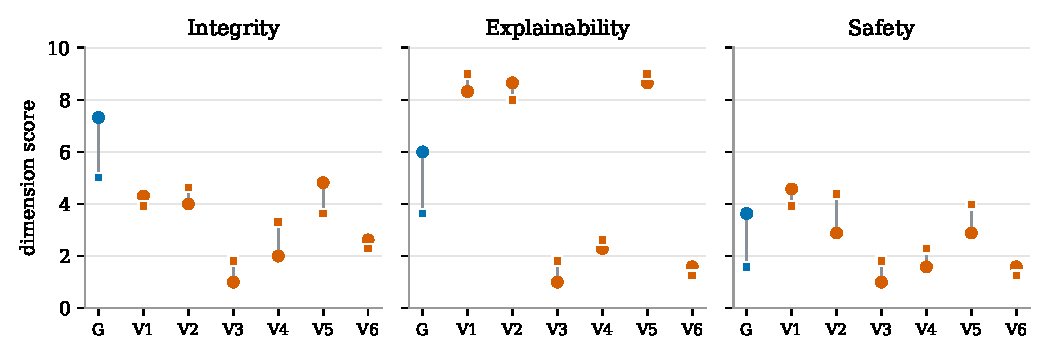
\includegraphics[width=\textwidth]{fig_variance.pdf}
\caption{Dimension scores in Run~1 (circles) and Run~2 (squares) for the three LLM-rated dimensions. Blue is the reference model; orange are the forged variants.}\label{fig:variance}
\end{figure}

The overall score changes by 0.05 to 0.49 points for the forged models and by 1.34 points for the reference model (Table~\ref{tab:variation}). The reference model's Integrity score dropped from 7.32 to 5.01, its Explainability score from 6.00 to 3.63 and its Safety score from 3.63 to 1.59, even though its card and metadata are the same in both runs. Spearman rank correlation of the seven overall scores between the two runs is 0.75. The ordering of the lowest three (V3, V4, V6 below the rest) is stable; the position of the reference model is not (first in Run~1, fourth in Run~2).

\begin{table}[H]
\centering\small
\caption{Overall FRIES score by run, and the difference.}\label{tab:variation}
\begin{tabularx}{\textwidth}{@{}p{3.8cm}RRRR@{}}
\toprule
\textbf{Model} & \textbf{Run 1} & \textbf{Run 2} & \textbf{Change} & \textbf{Rank (1 / 2)}\\
\midrule
G & 6.785 & 5.442 & $-$1.343 & 1 / 4\\
V1 & 6.562 & 6.487 & $-$0.076 & 3 / 2\\
V2 & 5.941 & 6.238 & +0.296 & 4 / 3\\
V3 & 3.864 & 4.354 & +0.490 & 7 / 6\\
V4 & 4.296 & 4.763 & +0.467 & 5 / 5\\
V5 & 6.672 & 6.723 & +0.051 & 2 / 1\\
V6 & 4.280 & 4.083 & $-$0.197 & 6 / 7\\
\bottomrule
\end{tabularx}
\end{table}

\paragraph{Determinism of the non-LLM path.} Within each run, the Fairness and Robustness metrics of V1 and V4 coincide exactly, and across runs those two dimensions never changed. This supports the claim that the probe pipeline itself is deterministic given a pinned seed.\label{sec:determinism}

\section{Testing hypotheses H1 and H2}
We compare each variant (Run~2) with the \emph{corrected} reference (Run~3), and also report the comparison with the original reference for completeness.

\begin{table}[H]
\centering\small
\caption{Hypothesis check against the corrected reference R*. ``Targeted dimension'' compares the variant's score on the dimension where its flaw was injected with R*'s score on that dimension. Overall scores: R* 6.16.}\label{tab:hyp}
\begin{tabularx}{\textwidth}{@{}p{1.3cm}p{2.5cm}RRRR@{}}
\toprule
\textbf{Variant} & \textbf{Dimension} & \textbf{R*} & \textbf{Variant (Run 2)} & \textbf{H1 holds?} & \textbf{Overall below R*?}\\
\midrule
V1 & Fairness & 7.32 & 6.60 & yes & no (6.49)\\
V2 & Robustness & 9.00 & 8.32 & yes & no (6.24)\\
V3 & Explainability & 6.65 & 1.82 & yes & yes (4.35)\\
V4 & Integrity & 3.91 & 3.30 & yes (small) & yes (4.76)\\
V5 & Safety & 3.91 & 3.98 & \textbf{no} & no (6.72)\\
V6 & Safety (and Expl.) & 3.91 & 1.26 & yes & yes (4.08)\\
\bottomrule
\end{tabularx}
\end{table}
For V6 we use Safety, one of its two injected flaws; its Explainability score (1.26) is also far below R*'s 6.65.

\textbf{H1} held for 5 of 6 variants against the corrected reference. The Integrity margin for V4 is 0.6 points, smaller than the run-to-run spread we observed for LLM-rated dimensions (Table~\ref{tab:variation}), so we would not call it a robust detection. The Robustness margin for V2 (8.32 against 9.00) is one band step, produced by a 3-point larger accuracy drop. V5 fails: its Safety score is 0.07 higher than R*'s. \textbf{H2} held for 3 of 6 (V3, V4, V6). The mean overall score of the six forged models is 5.44 against 6.16 for R*. Against the \emph{original} reference the figures are 6.79 and 5.44 (Runs~1 and~2), but we regard those comparisons as invalid for the Fairness and Robustness dimensions.

\section{Cost}
Evaluating the corrected reference (Run~3) took the same order of time. Fine-tuning one variant took about 160 s on the RTX 4060 laptop GPU. The seven evaluations of a run were created roughly 80--135 seconds apart (from the \code{created\_at} timestamps); this is an upper bound on one evaluation, including model loading, two inference passes over 3\,000 texts for the fairness and robustness probes, the perturbed pass, the LLM call and database writes. The result files do not record peak GPU memory or per-stage timings, so we do not report them. \todo{measure peak VRAM/RAM and per-stage time with a profiler and add here}

\chapter{Discussion}\label{ch:discussion}

\section{Does TrustLens identify the trustworthiness of a model?}
The honest answer from our data is: \emph{partly, and mostly for the part of trust that lives in documentation and metadata.}

\subsection{Evidence that supports the claim}
\begin{itemize}
\item \textbf{Documentation and integrity flaws were detected consistently.} V3, V4 and V6 had the three lowest overall scores in both runs, between 3.86 and 4.76, against 6.16 for the corrected reference. Their scores on the flawed dimension were below the reference's in every run.
\item \textbf{The behavioural fairness probe responded to a behavioural flaw.} The label-flipped model V1 produced a DPD of 0.42 with a confidence interval that excludes both the 0.32 of the unflipped V3 and the 0.28 of the corrected reference, and the Fairness score fell to 6.60 against 7.32. The probe is deterministic, and results for V1 and V4 (same weights) matched exactly.
\item \textbf{The compound model scored lowest overall in Run~2 and near the bottom in Run~1,} which matches the intuition that two flaws should score worse than one.
\item \textbf{Evidence is traceable.} For every number above there is a stored probe output with a hash, a rationale and a status. Even where we disagree with the score, we can see why it came out as it did. This is how we found the constant-predictor problem.
\end{itemize}

\subsection{Evidence against, and limits on the claim}
\begin{itemize}
\item \textbf{The safety flaw was not detected, and the overall score favoured three flawed models.} V5 under-flags severe toxicity, a genuine behavioural weakness, but the Safety probe never looks at behaviour. V5's card is complete and honest about the flaw, so the card-based probes rate it at least as well as the reference model, whose card is thin (Safety 3.98 against 3.91). In a sense the tool did what it was designed to do (reward disclosure) and that is exactly the problem: an honest card on a harmful model is rated above a sparse card on a possibly good model.
\item \textbf{The robustness flaw was only weakly visible.} V2 lost 4.1 points of accuracy under character swaps, four times the next variant and four times the corrected reference's 0.97, but the Robustness score moved only from 9.00 to 8.32 because the O/S/D band is dominated by accuracy, and the \code{R-ROB-PERT} trigger needs a 5-point drop.
\item \textbf{Three of five dimensions depend on an LLM and moved between runs.} The original reference model's overall score changed by 1.34 points between two evaluations of identical inputs, enough to change its rank from first to fourth. We evaluated the corrected reference only once, so its own spread is unknown.
\item \textbf{Our first reference evaluation was invalid, and we had to correct it.} The original Hub import behaved as a constant predictor, which gave it a perfect-looking Fairness and Robustness score. TrustLens did not warn about this. After converting the model to an equivalent two-label head, the reference scored Fairness 7.32 and Robustness 9.00 with a genuine demographic-parity gap of 0.28. The corrected comparison is the one we rely on, but it is a single evaluation, and the conversion itself (maximum probability difference $9.5{\times}10^{-4}$ on a four-sentence check) is a modelling step we introduced.
\item \textbf{Most of the signal comes from documents we wrote.} V3, V4 and V6 differ from clean models in their cards and licence fields. A forger who knows TrustLens could fix them in minutes.
\item \textbf{The experiment is small.} Seven models, one task, one dataset, one forger (us), two runs. We report counts and differences, not significance tests, because the sample cannot support them.
\end{itemize}

\subsection{Is it trustworthiness or an audit profile?}
We think the second description is more accurate. TrustLens produces an \emph{audit profile}: a structured record of what was measured, what was disclosed and what is missing, with a number attached that summarises a set of heuristic rules. The number is useful for sorting models that differ a lot in documentation quality, and it is not a measurement of trustworthiness in a sense that could be validated against ground truth, because no ground truth exists for the models in this experiment other than the flaws we ourselves injected. The project README makes the same claim about the score; we agree with it and would add that the evidence from Chapter~\ref{ch:results} supports the caution.

\section{Questions we asked of our own design}
\begin{description}[leftmargin=1.2em]
\item[Is FRIES sufficient?] No. It omits privacy, calibration, provenance beyond metadata, and environmental or legal aspects discussed in the surveys \cite{kemmerzell2025}. TrustLens implements five of many possible dimensions.
\item[Are the thresholds justified?] Not empirically. The README labels every metric-to-O/S/D band ``PROPOSED / REQUIRES VALIDATION''. $\varepsilon=0.05$, the 95\% intervals, the min-group size of 30 and the band formulas are design choices, not calibrated values.
\item[Could the difference come from something unrelated to trust?] Yes. Variants differ in training data size, class balance and learning rate as well as in the injected flaw, and the reference differs from them in architecture head and training data. Also, the integrity probe penalises the local variants for lacking a pinned revision and a manifest (\code{I-INT-REV-UNPINNED}, \code{I-INT-MANIFEST-MISSING}); those risks fire for \emph{every} variant because they are local directories and not Hub repositories, so part of the Integrity gap between the reference model and the variants reflects where the file lives and not what it contains.
\item[Does the overall score have statistical meaning?] No. It is a weighted mean of cube roots of integer ratings; the ratings are ordinal and partly LLM-generated.
\item[Could a malicious model evade the probes?] Easily. See Section~\ref{sec:threat}.
\end{description}

\section{Threats to validity}\label{sec:threats}
\paragraph{Internal validity.} Do the scores measure what we claim? For Fairness and Robustness, the metrics are well defined, but the reference model's mapping error shows that a valid-looking number can measure the wrong thing. Run~1 and Run~2 used slightly different integrity code, so we cannot attribute their differences to the LLM alone. We did not log the LLM provider and temperature per evaluation, and we could not check which provider answered. DPD conflates a true base-rate difference with model unfairness; the groups in the Civil Comments sample have different toxicity rates, which explains why the unflipped V3 still shows DPD 0.32.

\paragraph{External validity.} Seven models, one binary toxicity task, BERT-base variants, one dataset. Nothing here says how TrustLens behaves on image models, generative models, other languages, or models whose cards are well written but unfaithful. The robustness probe skips non-text models by design, and an earlier benchmark on six small models (documented in \code{docs/RESULTS\_SUMMARY.md}) found the same dimension skipped for two of them.

\paragraph{Construct validity.} FRIES as implemented measures: parity of predictions across one binary attribute; sensitivity to random typos; whether five card headings exist; whether metadata fields exist; whether four safety topics are mentioned. These are proxies. We do not show that they track the broader concept of trustworthiness, and the Safety and Explainability dimensions in particular are named after properties (preventing harm, explaining decisions) that the probes do not examine.

\paragraph{Reproducibility.} The data preparation, training and evaluation scripts are in the repository and the seeds, flip positions and hyperparameters are stored in manifests, so another researcher can rebuild the variants and the evaluation set. They cannot reproduce the LLM-rated dimensions exactly, because hosted models change and the provider is not pinned. The Fairness and Robustness dimensions reproduce exactly given the same weights and data, as the V1--V4 identity and the unchanged scores across runs show. We did not rerun the experiment on a second machine.

\section{Threat model}\label{sec:threat}
\begin{table}[H]
\centering\small
\caption{Threats an auditing tool would like to catch, and what TrustLens does about them in its current form.}
\begin{tabularx}{\textwidth}{@{}p{3.3cm}LL@{}}
\toprule
\textbf{Threat} & \textbf{What TrustLens does} & \textbf{What it cannot do}\\
\midrule
Misleading model card (over-claims, empty sections) & Detects missing sections and some contradictions; LLM judges content quality. & Cannot verify that a well-written card is true.\\
Missing or inconsistent licence/metadata & Integrity risks for unpinned revision, missing manifest, undisclosed licence. & Cannot judge legal compliance.\\
Tampered weights & Compares SHA-256 to a trusted reference \emph{if supplied}. & No reference was supplied in any experiment; hash-only checks cannot find backdoors in an unmodified-looking file whose hash is itself replaced.\\
Biased behaviour on a sensitive group & Measures DPD/EOD/F1 spread for one binary attribute with CIs. & Other attributes, intersections, and base-rate effects.\\
Fragility to input noise & Random character swaps. & Targeted or semantic attacks.\\
Unsafe outputs, missed harmful content & Checks that safety topics are disclosed. & Does not test behaviour at all.\\
Backdoors and poisoned behaviour \cite{gu2017badnets} & Nothing specific. & Not in scope.\\
Evaluator-aware adversary & Nothing. & A forger who reads the repository can write a card that passes every card check and train a model that behaves well on public probes.\\
\bottomrule
\end{tabularx}
\end{table}
TrustLens therefore does not provide complete model security. It is closer to a structured checklist with some measurements, useful as one input to a human reviewer.

\section{Lessons from building the forged models}
Three things surprised us. First, getting a model to be \emph{brittle} was harder than expected, because small or badly trained models collapse to the majority class and become stable. Second, the same effect meant that the reference model, through a mapping slip, also became stable and looked excellent. Third, the tool's most reliable detections were of flaws that we had put in the card, which suggests that the first useful role of such a tool is to check disclosure and metadata consistency, and the second, still to be built, is to run richer behavioural tests.

\chapter{Testing and Performance}\label{ch:testing}

\section{Testing strategy}
The backend has 85 files under \code{backend/tests} with 592 test functions by a simple count of \code{def test\_}; the worker package and the frontend have their own tests (Vitest for components such as the report, review and draft pages). Continuous integration (\code{.github/workflows/ci.yml}) runs \code{ruff check} and \code{pytest}, including a job that skips tests marked \code{integration}, and installs and tests the frontend with \code{npm ci}. We did not generate a coverage report for this thesis, so we cannot give a coverage percentage. \todo{run \code{pytest --cov} and insert line coverage}

\begin{table}[H]
\centering\small
\caption{Groups of automated tests (names from \code{backend/tests}).}
\begin{tabularx}{\textwidth}{@{}p{3.5cm}L@{}}
\toprule
\textbf{Area} & \textbf{Examples and what they check}\\
\midrule
Scoring & \code{test\_fries\_scorer}: cube-root, veto, aspect mean, weights; compares against frozen vectors in \code{shared/scoring/fixtures/fries\_test\_vectors.json} (shared with the frontend implementation).\\
Probes & \code{test\_fairness\_contract\_v2}, \code{test\_fairness\_stats}, \code{test\_robustness\_eval}, \code{test\_robustness\_nlp}, \code{test\_integrity\_probe}, \code{test\_explainability\_eval}, \code{test\_safety\_probe}, \code{test\_probe\_output\_contract}.\\
Inference & \code{test\_inference\_backend}, \code{test\_device\_resolution}, \code{test\_device\_placement}, \code{test\_model\_snapshot\_check}.\\
O/S/D engines & \code{test\_deterministic\_osd}, \code{test\_osd\_agent}, \code{test\_hybrid\_osd\_agent} (fallback on LLM failure), \code{test\_llm\_client}.\\
Pipeline and API & \code{test\_evaluation\_lifecycle}, \code{test\_e2e\_draft\_to\_report}, \code{test\_api\_reports}, \code{test\_report\_concurrency}, \code{test\_finalize\_modes}, \code{test\_human\_review}.\\
Honesty and migration & \code{test\_phase6\_honesty}, \code{test\_mode\_disclosure\_scoring\_state}, \code{test\_methodology\_version\_migration}, \code{test\_migration\_legacy\_readback}.\\
\bottomrule
\end{tabularx}
\end{table}

Most probe tests use injected fake backends rather than loading real models, so they check logic and contracts, not behaviour on real checkpoints. The forged-model experiment of Chapter~\ref{ch:results} is the only end-to-end test with real weights, and it found a problem that the unit tests could not (the label-mapping outcome). \todo{record the pass/fail counts of the latest full test run}

\section{What the tests do not cover}
There is no test that the heuristic bands produce sensible scores for a degenerate classifier, and no test comparing score ordering for a known good and a known bad model; the forged-model experiment is effectively the first such test. The original-reference problem shows the gap. We think the most valuable regression test to add is a smoke test that evaluates a constant predictor and expects a warning.

\section{Performance and resource use}
The system was run on the reference laptop: NVIDIA GeForce RTX 4060 Laptop GPU (8\,GB VRAM) with CUDA, float32, batch size 8. For a BERT-base classifier (109.5M parameters, 438\,MB on disk) this fits comfortably in VRAM. Measured costs are in the ``Cost'' section of Chapter~\ref{ch:results}: about 160\,s to fine-tune a variant and roughly 80--135\,s between consecutive finished evaluations. The README roadmap lists a resource checker and a benchmark-first runtime estimate as not yet implemented, so TrustLens does not currently predict whether a model will fit on the machine before loading it. Larger models would need that gate; for now, robustness may download and load a sequence-classification model at probe time with no memory check.

\chapter{Conclusion and Future Work}\label{ch:conclusion}

We close by answering the three questions we set out in Chapter~\ref{ch:intro}, one at a time, because they have different answers.

\section{Q1. Did we successfully implement TrustLens?}
Largely yes, within the scope we documented. The repository contains a working pipeline from Hub model import to local GPU inference, five probes, three O/S/D engines, the FRIES scorer verified against frozen vectors, human review, versioned reports, an evidence store and a dashboard, with 592 backend test functions. It does not contain several components that appear in our own target architecture: a resource checker, a benchmark-first runtime estimate, behavioural safety tests and SHAP/LIME explanations. Some probes are shallow, and the README itself lists ten known methodological gaps. The Explainability and Safety dimensions measure documentation only.

\section{Q2. Did TrustLens detect measurable differences between the reference and forged models?}
For some flaws, yes; for others, no. Against the corrected reference (overall 6.16), the score on the targeted dimension was lower for five of the six forged models (hypothesis H1): Fairness 6.60 against 7.32 with a clearly larger parity gap (0.42 against 0.28), Robustness 8.32 against 9.00, Explainability 1.82 against 6.65, Integrity 3.30 against 3.91 (a small margin), and Safety/Explainability 1.26 against 3.91 and 6.65 for the compound model. Models whose flaws lie in documentation and metadata (V3, V4, V6) also received clearly lower overall scores (4.08--4.76). On the other hand, the injected safety flaw (V5) was not detected (Safety 3.98 against 3.91), because the Safety probe does not examine behaviour; three of six forged models obtained a \emph{higher} overall score than the reference (H2 held for 3 of 6), and the LLM-rated dimensions varied between runs (1.34 points for the original reference). Our first reference evaluation was invalid because of a label-mapping error that made the model a constant predictor; the figures above use the corrected rerun.

\section{Q3. Does this prove that TrustLens can determine whether any arbitrary ML model is trustworthy?}
No, and our data points the other way in several respects. Seven models, one task, flaws that we designed, a single evaluation of the corrected reference, a probe set that did not flag a constant-predictor model, and LLM-rated dimensions that vary between runs do not support a general claim. Even a perfect separation of our seven models would show only that these probes can detect these flaws. TrustLens, in its current form, is best described as a \emph{structured, partly automated audit profile}: it records evidence about measurable properties and disclosure, it makes assumptions explicit, and its overall score is a convenient summary, not a validated measure of trust.

\section{Contributions, restated}
\textbf{Engineering:} the implemented system and its evidence discipline. \textbf{Methodological:} the three-layer separation and explicit evidence statuses. \textbf{Empirical:} a forged-model suite with manifests and a candid comparison, including a documented negative result for the Safety dimension and the discovery of the constant-predictor trap. \textbf{Future research opportunity:} validating any such score against independent judgments of trust.

\section{Future work}
Each item follows from a limitation reported above.
\begin{enumerate}
\item \textbf{Support multi-label heads natively} (a decision rule on a chosen output, instead of our head conversion) and add a probe-level warning when a model predicts a single class for (almost) every input; repeat the corrected reference evaluation several times to measure its spread.
\item \textbf{Behavioural safety probes.} A test set of harmful and benign prompts or comments, so that V5-style flaws change the Safety score.
\item \textbf{Pin and log the LLM,} set temperature to zero where possible, repeat each evaluation several times and report the spread. Alternatively replace the LLM step with a rule-based or human-reviewed mapping and compare.
\item \textbf{Stronger robustness attacks} (word-level and gradient-guided perturbations) and a band that does not depend on raw accuracy.
\item \textbf{Fairness beyond one attribute,} and a metric that separates base-rate differences from model bias.
\item \textbf{More models and more forgers:} dozens of Hub models with human trust ratings from at least two independent reviewers, multiple forged models built by people who did not write the probes, and statistical tests on the results. This is the only route to validating the score.
\item \textbf{Provenance.} Supplying trusted reference hashes, verifying model-card claims against evidence, and scanning for known backdoor patterns.
\item \textbf{Resource gating and runtime estimates} before loading weights, as specified but not yet built.
\item \textbf{Calibration of the confidence engine} and of the O/S/D bands against empirical data.
\end{enumerate}
None of these is implemented in the current repository.

\begin{thebibliography}{99}
\addcontentsline{toc}{chapter}{References}
\renewcommand{\bibname}{References}

\bibitem{rutinowski2024} J.~Rutinowski \emph{et al.}, ``Benchmarking Trust: A Metric for Trustworthy Machine Learning,'' in \emph{Explainable Artificial Intelligence (xAI 2024)}, Springer, 2024. (FRIES trust score.)

\bibitem{manzano2024} M.~Manzano, C.~Ayala, and C.~G\'omez, ``TrustML: A Python package for computing the trustworthiness of ML models,'' \emph{SoftwareX}, vol.~26, art.~101740, 2024.

\bibitem{vashistha2025} R.~Vashistha and A.~Farahi, ``I-trustworthy models: A framework for trustworthiness evaluation of probabilistic classifiers,'' in \emph{Proc.\ AISTATS}, 2025.

\bibitem{vashistha2024} R.~Vashistha and A.~Farahi, ``U-trustworthy models: Reliability, competence, and confidence in decision-making,'' arXiv:2401.02062, 2024.

\bibitem{kemmerzell2025} N.~Kemmerzell, A.~Schreiner, H.~Khalid, M.~Schalk, and L.~Bordoli, ``Towards a better understanding of evaluating trustworthiness in AI systems,'' \emph{ACM Computing Surveys}, 2025.

\bibitem{mattioli2024} J.~Mattioli \emph{et al.}, ``An overview of key trustworthiness attributes and KPIs for trusted ML-based systems engineering,'' \emph{AI and Ethics}, vol.~4, pp.~15--25, 2024, doi:10.1007/s43681-023-00394-2.

\bibitem{nist2023} National Institute of Standards and Technology, ``Artificial Intelligence Risk Management Framework (AI RMF 1.0),'' NIST AI 100-1, Jan.\ 2023.

\bibitem{mitchell2019} M.~Mitchell \emph{et al.}, ``Model cards for model reporting,'' in \emph{Proc.\ ACM FAT*}, 2019, pp.~220--229.

\bibitem{gebru2021} T.~Gebru \emph{et al.}, ``Datasheets for datasets,'' \emph{Communications of the ACM}, vol.~64, no.~12, pp.~86--92, 2021.

\bibitem{hardt2016} M.~Hardt, E.~Price, and N.~Srebro, ``Equality of opportunity in supervised learning,'' in \emph{Advances in Neural Information Processing Systems (NeurIPS)}, 2016.

\bibitem{borkan2019} D.~Borkan, L.~Dixon, J.~Sorensen, N.~Thain, and L.~Vasserman, ``Nuanced metrics for measuring unintended bias with real data for text classification,'' in \emph{Companion Proc.\ The Web Conference (WWW)}, 2019, pp.~491--500.

\bibitem{mehrabi2021} N.~Mehrabi, F.~Morstatter, N.~Saxena, K.~Lerman, and A.~Galstyan, ``A survey on bias and fairness in machine learning,'' \emph{ACM Computing Surveys}, vol.~54, no.~6, 2021.

\bibitem{ebrahimi2018} J.~Ebrahimi, A.~Rao, D.~Lowd, and D.~Dou, ``HotFlip: White-box adversarial examples for text classification,'' in \emph{Proc.\ ACL}, 2018, pp.~31--36.

\bibitem{ribeiro2020} M.~T.~Ribeiro, T.~Wu, C.~Guestrin, and S.~Singh, ``Beyond accuracy: Behavioral testing of NLP models with CheckList,'' in \emph{Proc.\ ACL}, 2020, pp.~4902--4912.

\bibitem{gu2017badnets} T.~Gu, B.~Dolan-Gavitt, and S.~Garg, ``BadNets: Identifying vulnerabilities in the machine learning model supply chain,'' arXiv:1708.06733, 2017.

\bibitem{jiang2023reuse} W.~Jiang \emph{et al.}, ``An empirical study of pre-trained model reuse in the Hugging Face deep learning model registry,'' in \emph{Proc.\ IEEE/ACM ICSE}, 2023.

\bibitem{devlin2019} J.~Devlin, M.-W.~Chang, K.~Lee, and K.~Toutanova, ``BERT: Pre-training of deep bidirectional transformers for language understanding,'' in \emph{Proc.\ NAACL-HLT}, 2019, pp.~4171--4186.

\bibitem{wolf2020} T.~Wolf \emph{et al.}, ``Transformers: State-of-the-art natural language processing,'' in \emph{Proc.\ EMNLP: System Demonstrations}, 2020, pp.~38--45.

\end{thebibliography}

\appendix
\chapter{Repository Map}
\begin{lstlisting}
backend/    FastAPI /v1, probes, O/S/D engines, FRIES scorer, reports, tests
worker/     Celery consumer (same probe pipeline)
frontend/   Vite + React dashboard (TypeScript)
configs/    pinned datasets and earlier benchmark configuration
docs/       methodology notes, runbook, earlier results write-up
results/    experiment outputs; flawed_model_suite/ holds this report's data
shared/     frozen FRIES scoring test vectors
report/     this LaTeX report and make_figures.py
\end{lstlisting}

\chapter{Contents of the Forged-Model Suite}
\begin{lstlisting}
results/flawed_model_suite/
  data/            eval_set.csv (3000 rows), per-variant training JSONL and manifests
  cards/           model card (README.md) of each variant
  models/          weights + train_manifest.json for variants 1-6 (+ the first V2 design)
  eval_results/    Run 1 JSON per model + _summary.json
  eval_results_v2/ Run 2 JSON per model + _summary.json
  eval_results_v3/ Run 3: corrected (2-label) toxic-bert, one evaluation
\end{lstlisting}
The evaluation set manifest records dataset \code{google/civil\_comments}, split \code{test}, seed 42, size 3000, positive rate 0.20, and thresholds 0.5 (toxicity) and 0.0001 (identity attack, severe toxicity).

\chapter{Corrected-Reference Run (Run 3)}
\begin{lstlisting}
python -m app.scripts.convert_reference_2label     # builds models/reference_toxicbert_2label
python -m app.scripts.run_reference_2label_eval    # one evaluation -> eval_results_v3/
\end{lstlisting}
Proposed O/S/D (Run 3): Fairness 7,7,8; Robustness 9,9,9; Integrity 3,4,5; Explainability 6,7,7; Safety 3,4,5; overall FRIES 6.16 (Fairness 7.32, Robustness 9.00, Integrity 3.91, Explainability 6.65, Safety 3.91).

\chapter{Raw Dimension Scores}
\begin{table}[H]
\centering\small
\caption{Dimension scores for both runs as stored in \code{\_summary.json} (rounded to two decimals).}
\begin{tabularx}{\textwidth}{@{}p{3.1cm}p{1.1cm}RRRRRR@{}}
\toprule
\textbf{Model} & \textbf{Run} & \textbf{F} & \textbf{R} & \textbf{I} & \textbf{E} & \textbf{S} & \textbf{FRIES}\\
\midrule
G & 1 & 8.65 & 8.32 & 7.32 & 6.00 & 3.63 & 6.79\\
G & 2 & 8.65 & 8.32 & 5.01 & 3.63 & 1.59 & 5.44\\
V1 & 1 & 6.60 & 9.00 & 4.31 & 8.32 & 4.58 & 6.56\\
V1 & 2 & 6.60 & 9.00 & 3.91 & 9.00 & 3.91 & 6.49\\
V2 & 1 & 5.85 & 8.32 & 4.00 & 8.65 & 2.88 & 5.94\\
V2 & 2 & 5.85 & 8.32 & 4.64 & 8.00 & 4.38 & 6.24\\
V3 & 1 & 7.32 & 9.00 & 1.00 & 1.00 & 1.00 & 3.86\\
V3 & 2 & 7.32 & 9.00 & 1.82 & 1.82 & 1.82 & 4.35\\
V4 & 1 & 6.60 & 9.00 & 2.00 & 2.29 & 1.59 & 4.30\\
V4 & 2 & 6.60 & 9.00 & 3.30 & 2.62 & 2.29 & 4.76\\
V5 & 1 & 8.00 & 9.00 & 4.82 & 8.65 & 2.88 & 6.67\\
V5 & 2 & 8.00 & 9.00 & 3.63 & 9.00 & 3.98 & 6.72\\
V6 & 1 & 6.60 & 9.00 & 2.62 & 1.59 & 1.59 & 4.28\\
V6 & 2 & 6.60 & 9.00 & 2.29 & 1.26 & 1.26 & 4.08\\
\bottomrule
\end{tabularx}
\end{table}

\chapter{Proposed O/S/D Triples}
\begin{table}[H]
\centering\small
\caption{O/S/D triples (O,S,D) per dimension as proposed by the \code{llm\_v1} engine, Run~2. Fairness and Robustness are heuristic bands; Integrity, Explainability and Safety are LLM-rated.}
\begin{tabularx}{\textwidth}{@{}p{2.2cm}LLLLL@{}}
\toprule
\textbf{Model} & \textbf{F} & \textbf{R} & \textbf{I} & \textbf{E} & \textbf{S}\\
\midrule
G & 9,9,8 & 8,8,9 & 7,6,3 & 3,4,4 & 1,2,2\\
V1 & 6,6,8 & 9,9,9 & 3,4,5 & 9,9,9 & 3,4,5\\
V2 & 5,5,8 & 8,8,9 & 4,5,5 & 8,8,8 & 3,4,7\\
V3 & 7,7,8 & 9,9,9 & 1,2,3 & 1,2,3 & 1,2,3\\
V4 & 6,6,8 & 9,9,9 & 3,3,4 & 2,3,3 & 2,2,3\\
V5 & 8,8,8 & 9,9,9 & 3,4,4 & 9,9,9 & 3,3,7\\
V6 & 6,6,8 & 9,9,9 & 2,2,3 & 1,1,2 & 1,1,2\\
\bottomrule
\end{tabularx}
\end{table}

\chapter{Regenerating the Report}
\begin{lstlisting}
cd report
python make_figures.py     # rebuilds figures/*.pdf from the result JSON files
tectonic main.tex          # or: pdflatex main.tex  (run twice for the table of contents)
\end{lstlisting}
Institution, supervisor and academic-year fields are macros at the top of \code{main.tex}. Passages marked \todo{...} in red need information that is not in the repository.

\end{document}
